% define documentclass
\documentclass[12pt, bibliography=totoc, a4paper, abstractoff, numbers=noenddot]{scrreprt}

% define used packages
\usepackage[left=4.0cm, right=2.0cm, top=3cm, bottom=3cm]{geometry}
\usepackage{bibgerm}
\usepackage[utf8]{inputenc}
\usepackage[T1]{fontenc}
\usepackage{graphicx}
\usepackage[ngerman]{babel}
\usepackage{lmodern}
\usepackage{listings}
\usepackage[numbers]{natbib}
\usepackage{acronym}
\bibliographystyle{alphadin}
\usepackage{float}

\usepackage{lastpage}

% advanced tables
\usepackage{array}

% header and footer
\usepackage{fancyhdr}

% links
\usepackage{url}

% internal links
\usepackage[colorlinks=true ,linkcolor=black,
			anchorcolor=black ,citecolor=black ,filecolor=black,
			menucolor=black ,urlcolor=black]{hyperref}

% mathematical formulas
\usepackage{amsmath, amssymb}

% fancy Diagrams %
\usepackage{tikz}
\usepackage{epstopdf}

% to include images side by side
\usepackage{subfigure}

% for nice bg on title page
\usepackage{eso-pic}
\newcommand\BackgroundPic{%
\put(0,0){%
\parbox[b][\paperheight]{\paperwidth}{%
\vfill
\centering
\includegraphics[width=\paperwidth,height=\paperheight,%
keepaspectratio]{images/Logo_H-BRS_background}%
\vfill
}}}

% define the programming language
\usepackage{listings}
\lstloadlanguages{Java,sh,bash,Haskell,HTML,PHP,XML}
\lstdefinelanguage{console}{
  morekeywords={},
  otherkeywords={warumgehtdasnicht>,\$}
}
\newcommand{\lstsetconsole}
{ \lstset{%language=sh,
        lineskip=-2pt,
        breaklines=true,
        language=console,
        breaklines=true,
        captionpos=b,
        commentstyle=\textit,
        keywordstyle=\bfseries,
        basicstyle=\ttfamily,
        stringstyle=\ttfamily,
        showstringspaces=false,
        frame=single,
        tabsize=2
  }
}
\lstdefinelanguage{scalaconsole}{
  morekeywords={},
  otherkeywords={scala>,\|}
}
\newcommand{\lstsetrepl}
{ \lstset{%language=sh,
        lineskip=-2pt,
        breaklines=true,
        language=scalaconsole,
        breaklines=true,
        commentstyle=\textit,
        keywordstyle=\bfseries,
        basicstyle=\ttfamily,
        stringstyle=\ttfamily,
        showstringspaces=false,
        frame=single,
        tabsize=2
  }
}
\newcommand{\lstsetjava}{
 \lstset{language=Java,
        breaklines=true,
        commentstyle=\textit,
        keywordstyle=\bfseries,
        basicstyle=\ttfamily,
        stringstyle=\ttfamily,
        showstringspaces=false,
        frame=single,
        captionpos=b,
        tabsize=2,
        literate=
        %linewidth=\textwidth,captionpos=b
        %numbers=left, stepnumber=5, numbersep=10pt
 }
}
\lstdefinelanguage{scala}{
  morekeywords={abstract,case,catch,class,def,%
    do,else,extends,false,final,finally,%
    for,forSome,if,implicit,import,lazy,match,mixin,%
    new,null,object,override,package,%
    private,protected,requires,return,sealed,%
    super,this,throw,trait,true,try,%
    type,val,var,while,with,yield},
  otherkeywords={_,:,=,=>,<-,<\%,<:,>:,\#,@},
  sensitive=true,
  morecomment=[l]{//},
  morecomment=[n]{/*}{*/},
  morestring=[b]",
  morestring=[b]',
  morestring=[b]"""
}
\newcommand{\lstsetscala}{
 \lstset{language=scala,
        breaklines=true,
        commentstyle=\textit,
        keywordstyle=\bfseries,
        basicstyle=\ttfamily,
        stringstyle=\ttfamily,
        showstringspaces=false,
        frame=single,
        tabsize=2
        %%linewidth=\textwidth,captionpos=b
        %numbers=left, stepnumber=5, numbersep=10pt
 }
}
\newcommand{\lstsethtml}{
 \lstset{language=HTML,
        breaklines=true,
        commentstyle=\textit,
        keywordstyle=\bfseries,
        basicstyle=\ttfamily,
        stringstyle=\ttfamily,
        showstringspaces=false,
        frame=single,
        tabsize=2
        %%linewidth=\textwidth,captionpos=b
        %numbers=left, stepnumber=5, numbersep=10pt
 }
}
\newcommand{\lstsetphp}{
 \lstset{language=PHP,
        breaklines=true,
        commentstyle=\textit,
        keywordstyle=\bfseries,
        basicstyle=\ttfamily,
        stringstyle=\ttfamily,
        showstringspaces=false,
        frame=single,
        tabsize=2
        %%linewidth=\textwidth,captionpos=b
        %numbers=left, stepnumber=5, numbersep=10pt
 }
}
\lstnewenvironment{code}
    {\lstset{}%
      \csname lst@SetFirstLabel\endcsname}
    {\csname lst@SaveFirstLabel\endcsname}
\newcommand{\lstsethaskell}{
    \lstset{
      language=Haskell,
      commentstyle=\textit,
      keywordstyle=\bfseries,
      basicstyle=\ttfamily,
      stringstyle=\ttfamily,
      showstringspaces=false,
      frame=single,
      flexiblecolumns=false,
      basewidth={0.5em,0.45em},
      literate={+}{{$+$}}1 {/}{{$/$}}1 {*}{{$*$}}1 {=}{{$=$}}1
               {==}{{$==$}}2 %{!=}{{$\not\equiv$}}2
               {>}{{$>$}}1 {<}{{$<$}}1 {\\}{{$\lambda$}}1
               {\\\\}{{\char`\\\char`\\}}1
               {->}{{$\rightarrow$} }2 {>=}{{$\geq$}}2 {<-}{{$\leftarrow$}}2
               {<=}{{$\leq$}}2 {=>}{{$\Rightarrow$} }2
               {\ .}{{$\circ$}}2 {\ .\ }{{$\circ$}}2 {(.)}{({$\circ$})}2
               {>>}{{>>}}2 {>>=}{{>>=}}2
               {|}{{$\mid$}}1
    }
}
\lstdefinelanguage{JavaScript}{
  keywords={typeof, new, true, false, catch,%
    function, return, null, catch, switch, var,%
    if, in, while, do, else, case, break},
  ndkeywords={class, export, boolean, throw, implements, import, this},
  sensitive=false,
  comment=[l]{//},
  morecomment=[s]{/*}{*/},
  morestring=[b]',
  morestring=[b]"
}
\newcommand{\lstsetjavascript}{
  \lstset{
		language=JavaScript,
		breaklines=true,
		commentstyle=\textit,
		basicstyle=\ttfamily,
		keywordstyle=\bfseries,
		stringstyle=\ttfamily,
		showstringspaces=false,
		frame=single,
		tabsize=2
  }
}
\newcommand{\lstsetxml}{
 \lstset{language=XML,
        breaklines=true,
        commentstyle=\sffamily,
        keywordstyle=\bfseries,
        basicstyle=\sffamily,
        showstringspaces=false,
        stringstyle=\ttfamily,
        frame=single,
        tabsize=2,
        literate=
        %linewidth=\textwidth,captionpos=b
        %numbers=left, stepnumber=5, numbersep=10pt
 }
}
\lstdefinelanguage{CSharp}{
 morekeywords = {abstract,event,new,struct,as,explicit,%
    null,switch,base,extern,object,this,bool,false,%
    operator,throw,break,finally,out,true,byte,fixed,%
    override,try,case,float,params,typeof,catch,for,%
    private,uint,char,foreach,protected,ulong,checked,%
    goto,public,unchecked,class,if,readonly,unsafe,%
    const,implicit,ref,ushort,continue,in,return,using,%
    decimal,int,sbyte,virtual,default,interface,sealed,%
    volatile,delegate,internal,short,void,do,is,sizeof,%
    while,double,lock,stackalloc,else,long,static,%
    enum,namespace,string,partial},
  morecomment = [l]{//},
  morecomment = [l]{///},
  morecomment = [s]{/*}{*/},
  morestring=[b]",
  sensitive = true
}
\newcommand{\lstsetcsharp}{
 \lstset{language=csharp,
        breaklines=true,
        commentstyle=\sffamily,
        basicstyle=\sffamily,
        keywordstyle=\bfseries,
        stringstyle=\ttfamily,
        showstringspaces=false,
        frame=single,
        tabsize=2
        %%linewidth=\textwidth,captionpos=b
        %numbers=left, stepnumber=5, numbersep=10pt
 }
}
\lstdefinelanguage{FSharp}{
  morekeywords={abstract,and,as,assert,base,begin,%
    class,default,delegate,do,done,downcast,downto,%
    elif,else,end,exception,extern,false,finally,for,fun,%
    function,if,in,inherit,inline,interface,internal,lazy,%
    let,match,member,module,mutable,namespace,%
    new,not,null,of,open,or,override,private,public,rec,%
    return,static,struct,then,to,true,try,type,upcast,use,%
    val,void,when,while,with,yield,asr,land,lor,lsl,lsr,lxor,%
    mod,sig,atomic,break,checked,component,const,%
    constraint,constructor,continue,eager,event,external,%
    fixed,functor,global,include,method,mixin,object,%
    parallel,process,protected,pure,sealed,tailcall,trait,virtual,volatile},     
  sensitive=false,
  morecomment=[l][\color{greencomments}]{///},
  morecomment=[l][\color{greencomments}]{//},
  morecomment=[s][\color{greencomments}]{{(*}{*)}},
  morestring=[b]"
}
\newcommand{\lstsetfsharp}{
 \lstset{language=fsharp,
        breaklines=true,
        commentstyle=\sffamily,
        basicstyle=\sffamily,
        keywordstyle=\bfseries,
        stringstyle=\ttfamily,
        showstringspaces=false,
        frame=single,
        tabsize=2
        %%linewidth=\textwidth,captionpos=b
        %numbers=left, stepnumber=5, numbersep=10pt
 }
}

%set default pagestyle
\pagestyle{empty}

\setlength{\parindent}{0pt}
\setlength{\parskip}{12pt}

\usepackage{tabularx}

% #####
% #
% # START config area
% #
% #####

\newcommand{\HEADER}[0]{H-BRS, WS 2018}
\newcommand{\PAGENUMBERS}[0]{\pagemark}
\newcommand{\DATE}[0]{\today}

\newcommand{\AUTHOR}[0]{Ben Kirsche}
\newcommand{\MATNR}[0]{9023848}
\newcommand{\STREET}[0]{Humperdinckstraße 20}
\newcommand{\ZIP}[0]{53721}
\newcommand{\TOWN}[0]{Siegburg}

\newcommand{\REFERENT}[0]{Prof. Dr. Harm Knolle}
\newcommand{\KOREFERENT}[0]{}

\newcommand{\TITLE}[0]{Anwendungsszenarien für Graphdatenbanken}
\newcommand{\COURSE}[0]{Studiengang Informatik}
\newcommand{\TYPE}[0]{Projektarbeit}
\newcommand{\COMPLETION}[0]{Master of Science}

% #####
% #
% # END config area
% #
% #####

% Hurenkinder und Schusterjungenregelung
\clubpenalty=100000
\widowpenalty=100000
\displaywidowpenalty=100000

% starting the document
\begin{document}

% set pagenumbering to roman(I II III IV)
\pagenumbering{Roman}
% input the title
% #####
% #
% # This is the titlelayout from Prof. Dr. Harm Knolle 
% # (Hochschule Bonn-Rhein-Sieg)
% #  
% #####

% #####
% #
% # Default layout
% #
% #####

%\AddToShipoutPicture*{\BackgroundPic}

\begin{titlepage}
  \begin{center}
  	
\includegraphics[scale=1]{./images/LogoH-BRS.jpg}
  \end{center}
  \vspace{40pt}
  \sffamily
  \begin{tabular}{|l>{\raggedright\hspace{0pt}\arraybackslash}p{15cm}}
    & \\
    & \large\textbf{\TYPE}\\[\baselineskip]
    & \huge\textbf{\TITLE}\\[\baselineskip]
    & - \COURSE\ -\\
    & \\
  \end{tabular}
  \vfill
  \begin{tabular}{ll@{}}
    & Fachbereich Informatik\\[\baselineskip]
    &   Referent: \REFERENT\\[\baselineskip]
    & \\[\baselineskip]
    & eingereicht von:\\[\baselineskip]
    & \AUTHOR\\[\baselineskip]
    & Matr.-Nr. \MATNR\\[\baselineskip]
    & \STREET\\[\baselineskip]
    & \ZIP \ \TOWN\\[\baselineskip]
    & \\[\baselineskip]
    & Sankt Augustin, den \DATE\\[\baselineskip]
  \end{tabular}
\end{titlepage}


\begin{abstract}
\section*{Zusammenfassung}\markboth{Zusammenfassung}{}
Im Rahmen der Master-Veranstaltung „Schemalose Datenbanken“ soll eine Ausarbeitung zum Thema  „Graphdatenbanken: Anwendungsszenarien und Implementierungen mit MariaDB-OQGRAPH“ erarbeitet werden. Zu diesem Zweck haben sich die drei Autoren zu der Arbeitsgruppe 1 zusammengeschlossen.

Die Ausarbeitung lässt sich in zwei grundsätzliche Teile gliedern. Der erste Teil ist von theoretischer Natur und betrachtet Anwendungsszenarien von Graphdatenbanken. Anhand einer breiten Auswahl von Business Cases soll nicht nur der Mehrwert von Graphdatenbanken in den entsprechenden Szenarien festgehalten, sondern auch eine Abgrenzung zu konkurrierenden, relationalen Ansätzen erörtert werden.

Folgende Szenarien werden vorgestellt:
\begin{itemize}
	\item Text-Mining, Natural Language Processing
	\item Soziale Netze
	\item Betrugserkennung
	\item Empfehlungs-Engine
	\item Verkehrsnetze
	\item Stammdatenmanagement
\end{itemize}

Der zweite Teil dieser Ausarbeitung wird eine praktische Umsetzung mittels MariaDB OQGRAPH \cite{oqgraph} sein. Zuvor wird noch das System, insbesondere seine Eigenheit, vorgestellt und die Installation auf dem Hochschulrechner dokumentiert.

Dieser Teil besteht aus zwei Anwendungen, die jeweils andere Anforderungen an eine Graphdatenbank stellen. Die erste Anwendung ist eine OLTP System in der Form eines Gästebuchs. Im Fokus steht dabei vor allem die Aspekte der Modellierung, dafür wird das eigentliche Modell in QOGRAP erstellt. Im Zuge dessen werden die Unterschiede, insbesondere die Vorteile, im Vergleich zu einem relationalem Ansatz erarbeitet. Des weiteren werden diverse Use Cases implementiert, die über ein eigens dafür entworfenes, simples Frontend gesteuert werden können.

Die zweite Anwendung ist ein einfaches soziales Netz, mit Nutzern und Kontakten. Hierbei handelt es sich um eine OLAP-System. Im Gegensatz zu der vorherigen Anwendung, wird hier die Modellierung nicht weiter beachtet. Der Fokus liegt stattdessen auf der Performance der Graphdatenbank. Betrachtet werden Projektion und Selektion über unterschiedliche Zugriffsmöglichkeiten, sowie Traversierung und Aggregation der Datensätze. Anhand diverser Metriken werden die Messungen evaluiert.
\nocite{*}
\end{abstract}


% load the preamble
% \renewcommand\abstractname{Danksagung}
\begin{abstract}
\section*{Vorwort}\markboth{Vorwort}{}
  \addcontentsline{toc}{chapter}{Vorwort}
\end{abstract}

% loads the fancy pagestyle for register part
% set the pagestyle to fancy
\pagestyle{fancy}

\fancyhf{}% clear all fields
  % define the header
  \fancyhead[L]{\leftmark}% left header
  \fancyhead[R]{\HEADER}% right header
  \renewcommand{\headrulewidth}{0.4pt}% top line

  % define the footer
  \fancyfoot[L]{\AUTHOR}% left footer
  \fancyfoot[R]{\pagemark}% right footer
  \renewcommand{\footrulewidth}{0.6pt}% bottom line

  % redefine the chaptermark to have '1. Chaptername' and not 'CHAPTER 1.
  % CHAPTERNAME'
  \renewcommand{\chaptermark}[1]{\markboth{\thechapter.\ #1}{}}

% override the plain style
\fancypagestyle{plain}{%
\fancyhf{}% clear all fields
  % define the header
  \renewcommand{\headrulewidth}{0.0pt}% top line

  % define the footer
  \fancyfoot[L]{\AUTHOR}% left footer
  \fancyfoot[R]{\pagemark}% right footer
  \renewcommand{\footrulewidth}{0.6pt}% bottom line
}


% create the registers
\tableofcontents
\newpage

% set pagenumbering to arabic(1 2 3 4)
\pagenumbering{arabic}
% loads the fancy pagestyle for main part
% set the pagestyle to fancy
\pagestyle{fancy}

\fancyhf{}% clear all fields
  % define the header
  \fancyhead[L]{\leftmark}% left header
  \fancyhead[R]{\HEADER}% right header
  \renewcommand{\headrulewidth}{0.4pt}% top line

  % define the footer
  \fancyfoot[L]{\AUTHOR}% left footer
  \fancyfoot[R]{\PAGENUMBERS}% right footer
  \renewcommand{\footrulewidth}{0.6pt}% bottom line

  % redefine the chaptermark to have '1. Chaptername' and not 'CHAPTER 1.
  % CHAPTERNAME'
  \renewcommand{\chaptermark}[1]{\markboth{\thechapter.\ #1}{}}

% override the plain style
\fancypagestyle{plain}{%
\fancyhf{}% clear all fields
  % define the header
  \renewcommand{\headrulewidth}{0pt}% top line

  % define the footer
  \fancyfoot[L]{\AUTHOR}% left footer
  \fancyfoot[R]{\PAGENUMBERS}% right footer
  \renewcommand{\footrulewidth}{0.6pt}% bottom line
}


\setcounter{secnumdepth}{4}

% #####
% # load the chapter from the files
% #####
\setcounter{chapter}{1}
\setcounter{section}{0}
\chapter{Anwendungsszenarien}
\section{Text-Mining, Natural Language Processing}
\section{Soziale Netze}
Unter dem Begriff Sozialem Netz versteht man eine Menge an Teilnehmern, häufig sind dies natürliche Personen, und verschiedenen Arten an Relationen zwischen diesen. Das durch die Beziehungen gebildete Netz lässt sich problemlos als Graph darstellen, indem die Teilnehmer als Knoten des Graphen dargestellt und die Beziehungen auf die Kanten abgebildet werden.

\begin{figure}
	\caption{Auschnitt aus Facebooks Socail-Graph: Checkin \cite{facebookTao}}
	\label{fig:fbCheckin}
	\centering
	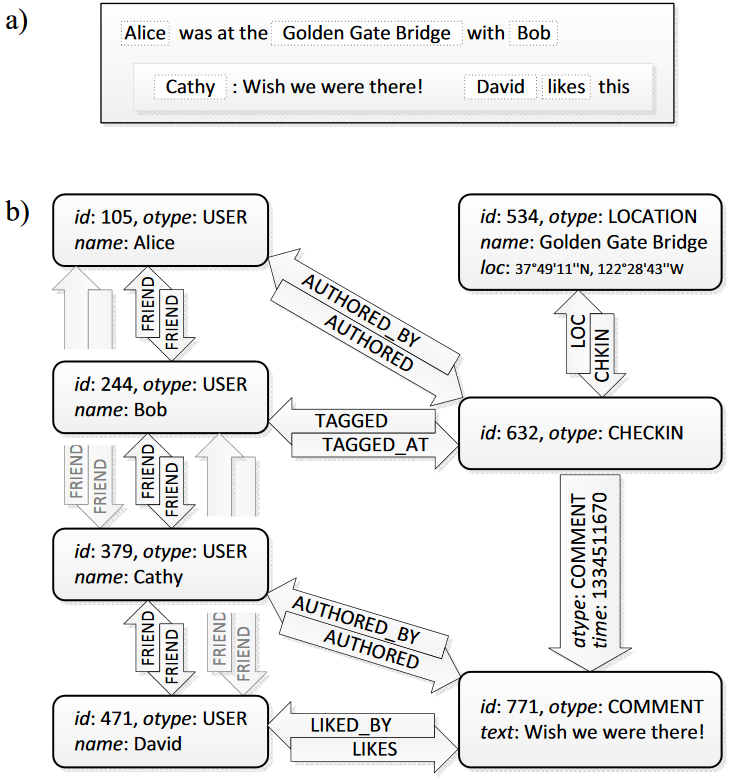
\includegraphics[width=0.7\textwidth]{images/facebook_checkin.png}
\end{figure}

Abbildung~\ref{fig:fbCheckin} zeigt beispielhaft wie ein Teil des Sozialen Netzes von Facebook aussieht. Anhand solcher Einträge wird für jeden einzelnen Nutzer eine personalisierte Startseite in Echtzeit erzeugt, dementsprechend wichtig ist ein performanter Datenzugriff. Um den Anforderungen gerecht zu werden hat Facebook eine eigene Graph-ähnliche API namens TAO entwickelt, welche den Datenbankzugriff effizient steuert. TAO stellt minimale Create/Update/Delete-Kommandos für Knoten und Kanten bereit. Der Großteil der Datenbankzugriffe ist allerdings lesend, folgende Querys sind möglich \cite{facebookTao}:
\begin{itemize}
	\item Alle Assoziation eines Typs zu einem Knoten
	\item Anzahl der Assoziationen eines Typs an einem Knoten
	\item Alle Nachbarn bis zur Tiefe n über eine bestimmte Assoziation
\end{itemize}
Dies ist ausreichend um mittels Verfahren wie Zentralitätsberechnung, Dichte und Cliquenanalyse für den Nutzer relevante Beiträge zu bestimmen \cite{sozialeNetzwerkanalyse}.


\section{Betrugserkennung}
Graph Datenbanken werden in e-commerce benutzt um die Betrug zu vermeiden. In Graph Datenbanken ist es möglich das Suchen der verdächtigen Pattern einzustellen - die entsprechenden Prüfungen, die mit den verschiedenen Triggern verbunden sind. Diese Triggern lassen sich die Probleme identifizieren, bevor als der ernschafte Schaden getroffen wird. Triggern können aus die nächste Ereignissen besteht werden: Einloggen in System, Registrierung einer neuen Bankkarte oder Bestellung der Waren.
\begin{figure}
	\caption{Transaktionsserie}
	\label{fig:Trs}
	\centering
	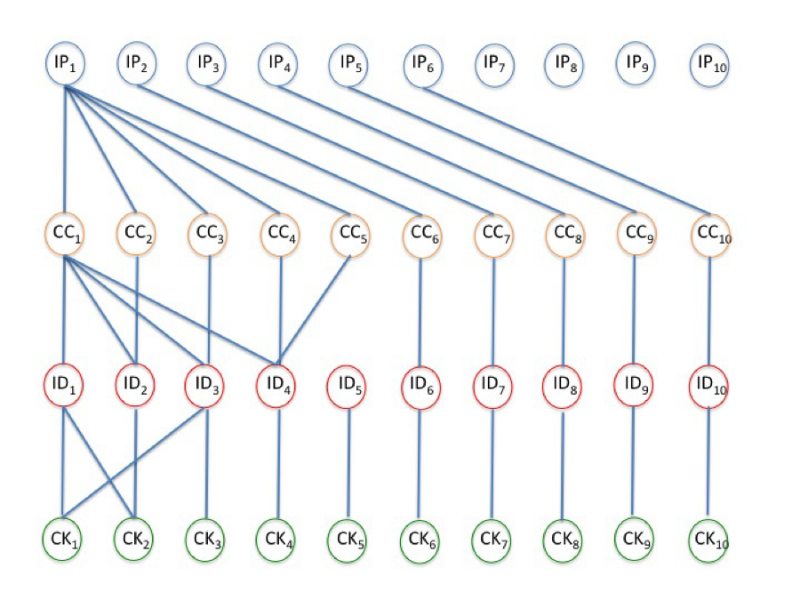
\includegraphics[width=0.7\textwidth]{images/Betrugserkennung.png}
\end{figure}

Auf der Abbildung~\ref{fig:Trs} sind die Transaktionsserien von den verschiedenen IP Adressen gezeigt. (IP(x) - IP Adresse, CC(x) - die Nummer der Kreditkarte, ID(x) - der Identifikator vom Nutzer, CK(x) - das Cookie, das im Systeme enthält). In diesem Beispiel ist es vermutlich, dass IP(1) von den Betrugen benutzt wird, denn vom IP(1) sind viele Transaktionen mit den unterschidliechen Kreditkarten durchgeführt, und eine Karte wurde von mehreren Nutzer benutzt, einige der auch mehr als eine Cookie besitzen. 
Graph Datenbanken sind die idealerweise Lösung der Bedrohungsentdeckung, die mit dem Finanzsicherheit in Netz verbunden sind, denn die Aktivität der Angreifern entspricht in jedem Fall zu einigen Pattern, und wenn sie rechtzeitig erkannt werden, können die möglichen Schaden minimiert werden.

\section{Empfehlungs-Engine}
Die Empfehlungsalgorithmen stellen die Verbindung zwischen den Leuten und den Dingen ein (die Waren, Dienstleistungen, Media-content) - alles, was relevant in diesem Bereich ist, wo diese Empfehlungsalgorithmen verwendet werden. Die Beziehungen werden basiert auf Benutzerverhalten. (Einkaufen, Bewertung, usw)
Die Effektivität der Empfehlungen hängt von dem Verstehen der Beziehungen zwischen Dingen ab und auch die Verbindung -qualität und -stärke. Diese Struktur ist am besten in Form von den attributierten Graphen vorgestellt. Die Anfragen in den Graphen sind meistens lokal, weil ihr Startpunkte ein oder einige identifizierte Objekte ist, und die weitere Suche ist in der Nähe von dieser Objekten durcgefürt.
Eine der ersten Empfehlungsalgorithmen war das System des Internet-Handels Amazon. Ein weiterentwickeltes Empfehlungsalgorithmus wurde von Google hergestellt. In diesem System war erstmal das Sammlungsverfahren der Nutzersinformationen verwendet worden, das cookies während der Besuchung der Suchmaschinen-Website benutzt wird und aufgrund der Suchensergebnisse wurde das Profil für jeden Nutzer aufgebaut.

\section{Verkehrsnetze}
\section{Stammdatenmanagement}
Stammdaten heißen die Daten, die kritisch wichtig für die Geschäftstransaktionen. Die Basisdaten enthält die Daten über die Benutzer, Einkäuferen, Produkten, Lieferanten, Abteilungen, Webseiten, usw. In den größen Organisationen sind solche Daten stark verteilt und heterogen nach den Formaten, Qualität und Zugangsmitteln. Das Stammdatenmanagement enthält die Identifizierung, Löschung, Speicherung und entsprechend Datenverwaltung. Das Stammdatenmanagement soll an der Veränderung der Oraganisationsstruktur, Verschmelzung von den Organisationen, Änderung der Geschäftsregeln usw. angepasst werden. Graph Datenbanken werden gut für die Modelirung, Speicherung, und Anfragen zu den Basismetadaten und Stammdatenmodellen gepasst werden. 



\newpage
\setcounter{chapter}{2}
\setcounter{section}{0}
\subsection{Installation}\label{Installation}
In diesem Kapitel wird die Installation und Konfiguration des DBS MaraiDB, sowie des Plugins QOGRAPH auf einem Ubuntu Rechner beschrieben.  
QOGRAPH wird als Plugin in einem eigenständigem Softwarepaket verteilt. Es ist nicht zwingend nötig den MariaDB-Server explizit zu installieren, dieser ist als Abhängigkeit definiert und wird automatisch mit installiert, wenn keine gültige Installation gefunden wird. Alle benötigten Pakete können mittels apt-get installiert werden.
\begin{lstlisting}
sudo apt-get install mariadb-plugin-oqgraph
\end{lstlisting}
Danach muss das Plugin noch installiert werden. Dafür in die DBMS-Konsole \texttt{mysql} wechseln und folgendes Kommando eingeben. Die Installation ist damit abgeschlossen.
\begin{lstlisting}
INSTALL SONAME 'ha_oqgraph';
\end{lstlisting}

Dabei ist zu beachten, dass MaraiDB das User-Directory von Unix nutzt. Dementsprechend kann nur mit root Rechten in die \texttt{mysql} Konsole  gewechselt werden. Es ist also nötig \texttt{sudo} zu verwenden. Damit auch normale User die Datenbank administrieren können, muss das \texttt{unix\_socket} Plugin deaktiviert werden.

\subsection{Visitenkarte}
\begin{enumerate}
	\item Allgemein
	\begin{enumerate}
		\item Name: MariaDB
		\item Modell: Storage Engines OQGRAPH
		\item Version: MariaDB 10.3.11, OQGRAPH 3.0
		\item Historie: MariaDB enstanden als Abspaltung (Fork) von MySQL, OQGRAPH als Plugin von MariaDB
		\item Hersteller: MariaDB Corporation, MariaDB Foundation
		\item Lizenz: GNU
		\item Quellen: https://mariadb.com/kb/en/library/documentation/, 
		https://dev.mysql.com/doc/internals/en/client-server-protocol.html
	\end{enumerate}
	\item Besonderheiten
	\begin{enumerate}
		\item Vergleichbare Systeme: MySQL
		\item Alleinstellungsmerkmale: OQGRAPH Grapherweiterung auf SQL Basis
	\end{enumerate}
	\item Architektur
	\begin{enumerate}
		\item Programmiersprache (des Systems): C, C++, Perl, Bash
		\item Systemarchitektur: InnoDB, Aria, OQGRAPH
		\item Betriebsart: Multi-User, Standalone, Cluster
		\item Protokoll der Schnittstelle: MySQL-Protocol
		\item API: SQL
	\end{enumerate}
	\item Datenmodell
	\begin{enumerate}
		\item Standardsprache: SQL
		\item Objektbegriff: Tabellen, Spalten, Zeilen, Attribute
		\item Sichten: Views
		\item Datentypen: Numeric, String, Date (in diversen Ausprägungen)
		\item Externe Dateien: BLOB (MEDIUMBLOB, LONGBLOB), TEXT (MEDIUMTEXT, LONGTEXT), JSON
		\item Schlüssel: Primär und Fremdschlüssel
		\item Semantisch unterschiedliche Beziehungen: Assoziation, Generalisierung, Spezifizierung
		\item Sonstige Constraints: Not Null, Check
	\end{enumerate}
	\item Indexe
	\begin{enumerate}
		\item Sekundärindexe: Plain Indexe, Full-Text Indexe
		\item Historische Daten: Transaktionsverwaltung, Logs
		\item Gespeicherte Prozeduren: SQL-Procedures
		\item Triggermechanismen: SQL-Trigger
		\item Versionierung: SYSTEM VERSIONING
	\end{enumerate}
	\item Anfragemethode
	\begin{enumerate}
		\item Kommunikation, Protokoll: MySQL-Protocol (TCP/IP)
		\item CRUD-Operationen: SQL (CREATE, INSERT, SELECT, UPDATE, ALTER, DELETE)
		\item Ad-hoc-Anfragen: Innerhalb spezieller Datenbank-Engines möglich (Casandra, ColumnStore)
		\item Kopplungstechniken: JOIN, UNION
		\item Map/Reduce: Nicht vorhanden
	\end{enumerate}
	\item Horizontale Skalierbarkeit
	\begin{enumerate}
		\item Konfiguration: Datenbank-Engine MaxScale
		\item Sharding: Spider, CONNECT oder Galera
		\item Replikation: GTID (Global Transaction Identifier), Master-Slave-Replikation
	\end{enumerate}
	\item Konsistenz
	\begin{enumerate}
		\item ACID: Erfüllt
		\item Transaktionen: SQL-Standard-Transactions
		\item Nebenläufigkeit (Synchronisation): Vorhanden
		\item Dauerhaftigkeit: Ja
		\item Konfliktbehandlung Replikation: Master-Slave-Replikation, Multi-Soruce-Replication
	\end{enumerate}
	\item Administration
	\begin{enumerate}
		\item Werkzeuge: PHPmyAdmin
		\item Massendatenimport: Load-Data-Infile, CONNECT-Engine
		\item Datensicherheit: Save-Data-Infile, MYSQL-Dump (Logisches Backup), MYSQl-Hotcopy (physikalisches Backup)
		\item Recovery: Engines XtraDB/InnoDB Recovery-Mode
		\item Komprimierung: Je nach Storage Engine
		\item Authentifizierung: In MariaDB integriert, Plugins: ed25519, GSSAPI, NamedPipe, PAM
		\item Mandantenfähigkeit: User und Rechtekonzept, getrennte Datenbanken
	\end{enumerate}
\end{enumerate}

\subsection{Grundlegende Funktionsweise des Systems}\label{chp:funktionsweise}
OQGRAPH ist ein Plugin, welches auf das normale relationale System von MariaDB aufbaut. Eine Graphdatenbank besteht prinzipiell lediglich aus zwei Tabellen. Eine Backing-Tabelle welche die Graphdaten in der Form von Kanten enthält und eine API-Tabelle auf die nur lesend zugegriffen werden kann. Diese zwei Tabellen werden im folgenden genauer beschrieben.

Die Backing-Tabelle ist eine normale relationale SQL Tabelle. Konkrete Anforderungen an diese bestehen nicht. Allerdings ist zu beachten das die API-Tabelle Daten aus Backing-Tabelle ließt und entsprechend gemappt werden muss. Damit dies gelingt muss die Tabelle jeweils eine \emph{not null numeric} Spalte für den Start- und Endknoten einer Kante bereitstellen. Es kann auch ein Kantengewicht gespeichert werden, OQGRAPH erwartet einen \emph{double} Wert. Darüber hinaus kann die Backing-Tabelle weitere beliebige Attribute enthalten. Es empfiehlt sich aber einen zusammengesetzten Primärschlüssel auf den beiden Kantenknoten zu definieren. Des Weiteren sorgt ein zusätzlicher Index auf dem Endknoten für optimale Performance bei den von OQGRAPH bereitgestellten Graphalgorithmen. Eine beispielhafte Implementierung des Schemas ist im Anhang \ref{schemaBacking} zu finden.

Die Api-Tabelle ist aus technischer Sicht ebenfalls nur eine SQL-Tabelle, ihre Aufgabe ist aber die Kapselung der datenhaltende Backing-Tabelle und das bereitstellen diverser Graphalgorithmen. Das Schema dieser Tabelle ist komplett vorgegeben und muss so übernommen werden, eine entsprechende Vorlage ist Anhang \ref{schemaApi} zu finden. Auf dieser Tabelle können mittels SQL-Syntax Graphalgorithmen durchgeführt werden. Die geschieht über ein Select auf der API-Tabelle, über die Where-Klausel können Argumente an die Algorithmen übergeben werden. Das Latch Attribut bestimmt den konkreten Algorithmus, \emph{origid} und \emph{destid} sind die Start und Endpunkte. In der folgenden Tabelle sind alle von OQGRAPH bereitgestellten Operationen aufgelistet.

\begin{tabularx}{\textwidth}{l l X}
	\textbf{Latch Wert }    & \textbf{Where-Klausel}  & \textbf{Graphoperation} \\
	\hline
	(empty string) & origid         & List all first hop vertices from origid in linkid column. \\
	dijkstras      & origid, destid & Find shortest path using Dijkstras algorithm between origid and destid, with traversed vertex ids in linkid column. \\
	dijkstras      & origid         & Find all vertices reachable from origid, listed in linkid column, and report sum of weights of vertices on path to given vertex in weight. \\
	dijkstras      & destid         & Find all vertices from which a path can be found to destid, listed in linkid column, and report sum of weights of vertices on path to given vertex in weight. \\
	breadth\_first & origid         & List vertices reachable from origid in linkid column. \\
	breadth\_first & destid         & List vertices from which a path can be found to destid in linkid column. \\
	breadth\_first & origid, destid & Find shortest path between origid and destid, report in linkid column. \\
	leaves         & origid         & List vertices reachable from origid, that only have incoming edges. \\
	leaves         & destid         & List vertices from which a path can be found to destid, that only have outgoing edges.
\end{tabularx}



\newpage
\setcounter{chapter}{3}
\setcounter{section}{0}
In diesem Kapitel wird beschrieben wie das semantische Schema einer typische OLTP-Anwendung, also ein System welches traditionell mit relationalen Datenbanken arbeitet, in ein Graph-Schema von MariaDBs OQGRAPH überführt werden kann. Als Beispiel dient ein Diskussionsforum, in dem Mitglieder Beiträge verfassen und kommentieren können. Abbildung \ref{fig:semanticSchema} zeigt das semantische Schema des Forums. In den folgenden Abschnitten wird das ensprechnde Datenbankschema konzipiert, sowie diverse typische Usecases für ein solches Forum erläutert und implementiert. Die Verwendung dieser Usecases erfolgt über einem entferntem PHP-Client, welcher ebenfalls kurz vorgestellt wird.

\begin{figure}[h]
	\centering
	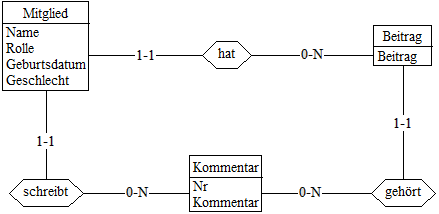
\includegraphics[width=0.6\textwidth]{images/semantischesSchema.png}	
	\caption{Semantisches Schema der Beispielwendung: Diskussionsforum}
	\label{fig:semanticSchema}
\end{figure}

\subsection{Konzeption des Schema}
OQGRAPH wird als Engine beschrieben, welche dem Nutzer die Handhabung hierarchische Strukturen (Bäume) und komplexe Graphen (zahlreiche Kanten) ermöglichen soll \cite{oqgraph}. Dieser Aussage wird OQGRAPH, insbesondere im erstem Punkt, nicht gerecht. Die Grundlegende Funktionsweise des Systems wird in Kapitel \ref{chp:funktionsweise} beschrieben.

Das Kernproblem von OQGRAPH, welches die Modellierung hierarchischer Strukturen betrifft, ist das Knoten nicht, beziehungsweise nicht explizit gespeichert werden. Lediglich ein numerischer Wert welcher den Knoten repräsentiert wird vorgehalten. Die resultiert in zwei Problemen. Zum einen kann nicht zwischen unterschiedlichen Knotenausprägungen (z. B. Kommentar und Beitrag) unterschieden werden. Dementsprechend ist es auch nicht möglich Knoten bei der Traversierung zu filtern. 

Zum anderen werden die Knoten in OQGRAPH durch eine globale Objektinstanz repräsentiert. Relationale Schema arbeiten aber typischerweise mit einen lokalen Identifikator. Das heißt es ist ein explizites Mapping nötig, wenn der OQGRAPH Knoten mit dem zugehörigen Nutzdatensatz in Verbindung gebracht werden soll. Möchte man diese Daten also zusammenführen ist ein Join notwendig. Graphdatenbanken sind aber so performant weil es eben nicht nötig ist Datensätze zu über einen Join zusammenzuführen.

Aufgrund dieser Limitierungen ist OQGRAPG ungeeignet für die Umsetzung komplexer Schemata. Um dies weiter auszuführen wurde ein OQGRAPH kompatibles Schema erstellt. In wie fern damit Usecases umgesetzt werden können, beziehungsweise wie Workarounds aussehen und mit Limitierungen umzugehen ist, wird in den folgenden Abschnitten vorgestellt.

Abbildung \ref{fig:logicSchema} zeigt das konzeptionelle Schema unserer Beispielanwendung Diskussionsforum. Die drei Objekte Mitglied, Benutzer und Kommentar werden in relationalen Tabellen gespeichert und bekommen einen lokal gültigen Primärschlüssel. Aber anstatt eines Fremdschlüssels auf die entsprechende Beziehungstabelle halten diese eine global eindeutige Objektidentität vor welche in der Backing-Tabelle von OQGRAPH verwendet werden. Dieser Identifier wird durch eine separate Sequenz verwaltet, ein Index auf diesem ermöglicht des Weiteren schnelles Auffinden der Nutzdaten zu den von dem Graphalgohritmus gefundenen Ergebnissen. Die Relationen werden also als Kanten durch das OQGRAPH verwaltet, zu den eigentlichen Kanten (Start/Endknoten, Gewicht) wird auch Relationstyp gespeichert, so das bekannt ist welcher Ausprägung der Zielknoten hat und so die Nutzdaten direkt aus der entsprechenden Tabelle geladen werden können. Da die referenzierte Nutzdatentabelle über den Relationstyp aufgelöst werden muss, kann auch nicht durch die DB referentielle 
Integrität gewährleistet werden.

\begin{figure}	
	\centering
	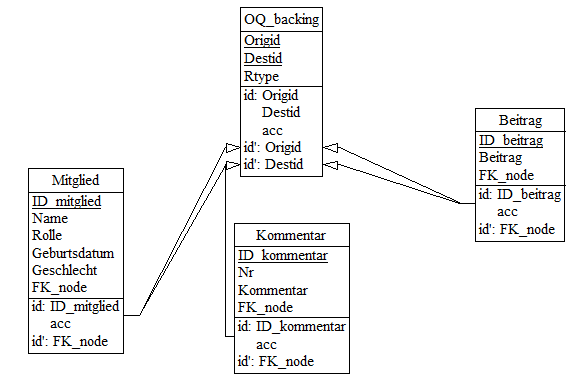
\includegraphics[width=0.9\textwidth]{images/logischesSchema.png}
	\caption{Logisches Schema der Beispielwendung: Diskussionsforum}
	\label{fig:logicSchema}
\end{figure}
 
Das komplette SQL-Schema, sowie des Installationsprotokoll auf dem Hochschulrechner, ist im Anhang \ref{todo} zu finden.

\subsection{Umsetzung eines Clients}
Bei der Entwicklung eines Clients für die Graph-Datenbank des Gästebuchsystems wurde sich für eine Webanwendung entschieden. Webanwendungen können über den Webbrowser aufgerufen und genutzt werden. Sie stehen damit einer Vielzahl von Nutzern zur Verfügung. Ein weiter Vorteil von Webanwendungen ist, dass die Entwicklung des User Interfaces nicht sehr aufwendig ist. Es müssen lediglich gängige Technologien der Webentwicklung für User Interfaces herangezogen werden, die dann schließlich vom Webbrowser interpretiert werden.

Der Client teilt sich auf in die die server-seitige Datenbereitstellung, sowie der client-seitige Datendarstellung.

\subsubsection{Datenbereitstellung}
Die Datenbereitstellung hat die Aufgabe mit der Datenbank zu kommunizieren und die Daten für die Datendarstellung aufzubereiten. Zur Entwicklung der Datenbereitstellung wurde die Skriptsprache PHP gewählt. Bei der Architektur des Systems wurde auf das im Software Engineering gängige Model-View-Control-Pattern (MVC) zurückgegriffen.

Neben den verschiedenen MVC-System-Komponenten ist die Datenbank-Kommunikation eine sehr wichtige Service-Komponente. Bei dem \grqq mysqlConnect\grqq{} handelt es sich um die PHP-Klasse, die die Kommunikation mit der Datenbank abwickelt. Dabei nutzt die mysqlConnect-Klasse die MySQLi-Erweiterung von PHP \cite{PHP-Mysqli}. Eine Erweiterung von PHP im speziellen für MariaDB oder sogar für die Store-Enginge OQGRAPH gibt es nicht. Dafür ermöglicht die MySQLi-Erweiterung das Absetzen von regulären, aber auch von OQGRAPH entsprechende SQL-Befehle \cite{PHP-Mysqli-Query}. Neben der Ausführung diverser SQL-Befehle unterstützt die MySQLi-Erweiterung auch die Interpretation der Antwort der Datenbank. Sogenannte Fetch-Operationen lesen dabei alle Zeilen der Antwort-Tabelle ein und erlauben damit PHP eine Verarbeitung der entsprechenden Zeilen \cite{PHP-Mysqli-Fetch}.

Als Service-Komponente bietet die mysqlConnect-Klasse den Service der Kommunikation mit der Datenbank an. Sie ist in der Datenbereitstellung die einzige Stelle, die eine Kommunikation mit der Datenbank erlaubt. Das bedeutet also auch, dass sich die Nutzer der mysqlConnect-Klasse nicht mehr um die datenbank-spezifische Kommunikation kümmern müssen. Dafür muss die mysqlConnect-Klasse aber auch alle nötigen Zusicherungen erfüllen, da sich die Nutzer unter Angabe von Parametern darauf verlassen müssen, dass sie die gewünschten Daten erhalten. Solange diese Zusicherung erfüllt wird ist es für den Nutzer nicht relevant wie genau die Zusicherung implementiert wird. So kann beispielsweise die Kommunikationsart oder gar die ganze Datenbank ausgetauscht werden, ohne dass Änderungen im übrigen System notwendig werden. Änderungen im Schema der Datenbank betreffen so beispielsweise allein die mysqlConnect-Klasse. Hierbei handelt es sich also um das Adapter-Pattern.

Die mysqlConnect-Klasse beinhaltet alle Operationen bezüglich des CREATE, READ, UPDATE und DELETE (CRUD) in Bezug auf Mitglieder, Beiträge und Kommentare. Darüber hinaus besitzt die mysqlConnect-Klasse speziellere Leseoperationen, bspw. im Bezug auf die Kantenbeziehungen zwischen einzelnen Knoten. Für die Datenbereitstellung wurden jedoch keine Funktionen von OQGRAPH genutzt (siehe \ref{OQGRAPH-Client} \nameref{OQGRAPH-Client}).

\begin{figure}	
	\centering
	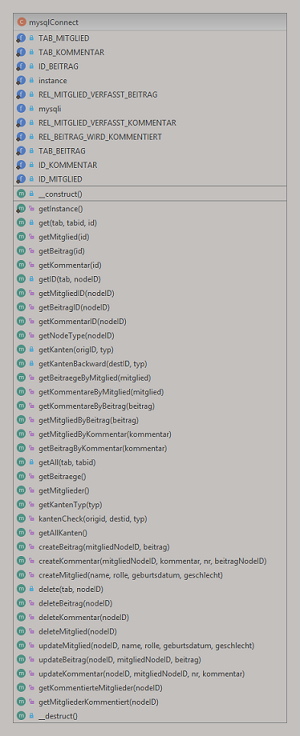
\includegraphics[width=0.6\textwidth]{images/mysqlConnect2.png}
	\caption{UML-Diagramm der Klasse \grqq mysqlConnect\grqq{} (erstellt mit PHPStorm)}
\end{figure}

Die verschiedenen Knoten Mitglieder, Beiträge und Kommentare sind als Model-Klassen implementiert worden. Aus ihnen können Objekte generiert werden, die die jeweiligen Elemente, aber auch die Knoten darstellen. Für die Erstellung des Objektes wird die jeweilige Objekt-ID benötigt. Sollte nur die jeweilige Knoten-ID vorliegen, kann mittels des mysqlConnect-Adapters die zugehörige Objekt-ID ermittelt werden.

Die View-Komponenten liefern die nötigen Informationen an die Datendarstellung. Hierfür nutzen die View-Komponenten den mysqlConnect-Adapter, sowie die verschiedenen Model-Klassen und den darauß resultierenden Objekten. Sie bieten der Darstellungen unter anderem die CRUD-Operationen auf die Graph-Datenbank an, dessen Anfragen und Aufgaben an den mysqlConnect-Adapter weitergereicht werden. Die verschiedenen View-Komponenten resultieren aus den entsprechenden Use Cases, die in \ref{Datendarstellung} \nameref{Datendarstellung} beschrieben werden.

\subsubsection{Datendarstellung}\label{Datendarstellung}

Die Datendarstellung teilt sich in die Sicht der Beiträge und Kommentare, sowie in die Sicht eines einzelnen Mitgliedes auf. Die Sicht der Beiträge und Kommentare listet alle aktuellen Beiträge auf und stellt zu jedem Beitrag seine Kommentare dar. In dieser Sicht ist es ebenso möglich, Beiträge und Kommentare, aber auch Mitglieder zu erstellen. Die Sicht eines einzelnen Mitgliedes stellt die Informationen und Statistiken über das einzelne Mitglied dar. Beide Sichten erfüllen dabei einige der im Projektplan dargelegten Use Cases.

Bei der Entwicklung der Sichten wurden Webkomponenten entwickelt. Bei Webkomponenten handelt es sich um JavaScript-Objekte, die vom Webbrowser interpretiert werden und deswegen dynamisch geladen, erzeugt und aktualisiert werden können. Dabei nutzen die Webkomponenten beim Laden der Webseite die View-Komponenten der Datenbereitstellung, um darzustellende Informationen zu erhalten, zu speichern und anzuzeigen.

Eine Webkomponente stellt dabei unter anderem einen einzigen Beitrag oder einen Kommentar dar. Diese Webkomponenten werden durch speziell definierte HTML-Tags und der jeweiligen Objekt-ID generiert. Es gibt aber auch Webkomponenten für das Erstellen, Bearbeiten, Ansehen und Löschen von Mitgliedern, Beiträgen und Kommentaren.

Folgende Use Cases wurden umgesetzt:
\begin{itemize}
	\item \textbf{Einfügen neuer Mitglieder, Beiträge und Kommentare}: Hierfür werden die Webkomponenten \grqq gb-neu-beitrag.js\grqq{}, \grqq gb-neu-kommentar.js\grqq{} und \grqq gb-neu-mitglied.js\grqq{} genutzt. Für das Erstellen der jeweiligen Elemente werden die View-Komponenten \grqq createBeitrag.php\grqq{}, \grqq createKommentar.php\grqq{} und \grqq createMitglied.php\grqq{} genutzt. Für das Erstellen von Beiträgen und Kommentaren ist das entsprechende Mitglied notwendig. Die Webkomponenten für das Erstellen von Beiträgen und Kommentaren erhalten die entsprechenden Mitglieder von den View-Komponenten \grqq getMitglied.php\grqq{} und \grqq getMitglieder.php\grqq{}. Die Webkomponenten werden in der Sicht für Beiträge und Kommentare genutzt. Das Erstellen von Kommentaren ist aber auch in der Sicht über einzelne Mitglieder möglich.
	\item \textbf{Löschen von Mitglieder, Beiträge und Kommentare}: Die Webkomponenten \grqq gb-beitrag.js\grqq{} und \grqq gb-kommentar.js\grqq{} beinhalten einen Button, mittels dem der zugehörige Beitrag oder Kommentar gelöscht werden kann. Das Löschen von Beiträgen und Kommentaren ist sowohl in der Sicht für Beiträge und Kommentare, als auch in der Sicht über einzelne Mitglieder möglich. Für das Löschen von Mitgliedern gibt es eine eigene Webkomponente \grqq gb-loeschen-mitglied.js\grqq{} in der Sicht von Beiträgen und Kommentaren. Für das Löschen werden die View-Komponenten \grqq deleteBeitrag.php\grqq{}, \grqq deleteKommentar.php\grqq{} und \grqq deleteMitglied.php\grqq{} entsprechend genutzt.
	\item \textbf{Ändern von Mitgliedern, Kommentaren und Beiträgen}: Hierfür werden in den Webkomponenten \grqq gb-beitrag.js\grqq{} und \grqq gb-kommentar.js\grqq{} Buttons zur Bearbeitung angeboten. Außerdem bietet die Webkomponente \grqq gb-loeschen-mitglied.js\grqq{} nicht nur eine Option für das Löschen, sondern auch für das Bearbeiten von Mitgliedern an. Die tatsächliche Bearbeitung findet dann in den Komponenten \grqq gb-neu-beitrag.js\grqq{}, \grqq gb-neu-kommentar.js\grqq{} und \grqq gb-neu-mitglied.js\grqq{} statt, die dann zur Bearbeitung umfunktioniert werden. Zur Speicherung der Änderung werden die View-Komponenten \grqq updateBeitrag.php\grqq{}, \grqq updateKommentar.php\grqq{} und \grqq updateMitglied.php\grqq{} genutzt.
	\item \textbf{Anzeige und Anzahl der Kommentare ausgewählter Beiträge}: Die Webkomponente \grqq gb-beitrag.js\grqq{} stellt einen einzelnen Beitrag dar. Dazu führt es auch die zugeordneten Kommentare mit der Webkomponente \grqq gb-kommentar.js\grqq{} auf. Es nutzt dafür unter anderem die View-Komponenten \grqq getBeitrag.php\grqq{}, \grqq getKommentar.php\grqq{}, sowie \grqq getMitglied.php\grqq{}.
	\item \textbf{Anzeige und Anzahl der Beiträge ausgewählter Mitglieder}: In der Sicht über einzelne Mitglieder werden dessen Beiträge aufgelistet, sowie deren Anzahl aufgeführt. Hierfür wird die Webkomponente \grqq gb-mitglied-beitraege.js\grqq{} genutzt, die wiederum die View-Komponenten \grqq getBeitraegeByMitglied.php\grqq{} nutzt. Für das Anzeigen der Beiträge wird die Webkomponente \grqq gb-beitrag.js\grqq{} genutzt.
	\item \textbf{Anzeige und Anzahl der Kommentare ausgewählter Mitglieder}: Ebenfalls in der Sicht über einzelne Mitglieder werden die Beiträge aufgelistet, die vom jeweiligen Mitglied kommentiert wurden. Hierbei wird auch in der Anzahl der Beiträge und der Anzahl der Kommentare des jeweiligen Mitgliedes differenziert. Hierzu nutzt die Webkomponente \grqq gb-mitglied-kommentar.js\grqq{} die View-Komponente \grqq getKommentareByMitglied.php\grqq{}. Für das Anzeigen der Beiträge wird die Webkomponente \grqq gb-beitrag.js\grqq{} genutzt.
	\item \textbf{Anzeige und Anzahl der kommentierten Beiträge ausgewählter Mitglieder}: Dies wurde bereits im Use Case \grqq Anzeige und Anzahl der Beiträge ausgewählter Mitglieder\grqq{} umgesetzt.
	\item \textbf{Anzeige Anzahl der kommentierten Mitglieder ausgewählter Mitglieder}: Hierfür werden zwei Statistiken angezeigt:
	\begin{enumerate}
		\item Eine Statistik die anzeigt, wie oft das jeweilige Mitglied von einem anderen Mitglied kommentiert wurde. Hierzu wird die Webkomponente \grqq gb-mitglied-von-mitglied.js\grqq{} genutzt, die ihre Informationen von der View-Komponente \grqq getKommentareMitgliedVonMitglied.php\grqq{} erhält. Sie listet zu jedem Mitglied auf, welches Mitglied wie oft das jeweilige Mitglied kommentiert hat.
		\item Eine Statistik darüber, wie oft das jeweilige Mitglied andere Mitglieder kommentiert hat. Die Webkomponente \grqq gb-mitglied-mitglied.js\grqq{} zeigt die Informationen der View-Komponente \grqq getKommentareMitgliedZuMitglied.php\grqq{} an. Dabei gibt die Statistik zu jedem Mitglied die Anzahl der Kommentare an, die das jeweilige Mitglied bei Beiträgen des angegebenen Mitglieds hinterlassen hat.
	\end{enumerate}
\end{itemize}

\subsubsection{OQGRAPH im Bezug auf den Client}\label{OQGRAPH-Client}

Die Funktionalitäten von OQGRAPH wurden bei der Entwicklung des Clients nicht genutzt. Die Gründe dafür sind vielseitig. Zum einen war die Nutzung von OQGRAPH in diesem Anwendungsfall nicht sinnvoll, weil OQGRAPH keine Möglichkeit bietet zwischen einzelnen Knoten-Arten und Kanten-Beziehungen zu unterscheiden. Eine Selektion von Beitragsknoten ist über Funktionalitäten von OQGRAPH nicht möglich - hierfür muss ein reguläres SQL herangezogen werden. Rückschlüsse auf Knoten-Arten sind zwar in der Theorie über die Gewichte der Wege möglich, jedoch nicht immer sinnvoll und aussagekräftig.

Zum anderen ist auch OQGRAPH in einer relationalen Datenbank \grqq gefangen\grqq{}. So gibt es die erreichbaren Knoten, jedoch nicht den Weg an. Beispielsweise wäre bei der Statistik \grqq Mitglied wurde von anderes Mitglied so oft kommentiert\grqq{} der Pfad essentiell, da nur so ermittelt werden kann wie oft ein Mitglied das andere kommentiert hat. Durch die SQL-Erweiterung von OQGRAPH ist es so nur möglich festzustellen, dass ein Mitglied ein anderes kommentiert hat - jedoch nicht, wie oft.

Ein Beispiel aus den Testdaten verdeutlicht das Problem. Das Mitglied \grqq Oliver Higgins\grqq{} hat drei Beiträge verfasst, die insgesamt elf mal kommentiert wurden. Zwei Kommentare davon kommen vom Mitglied \grqq Leon Clemens\grqq{}. Dabei kommentierte Leon Clemens zwei Beiträge jeweils einmal.

\begin{figure}[h]
	\centering
	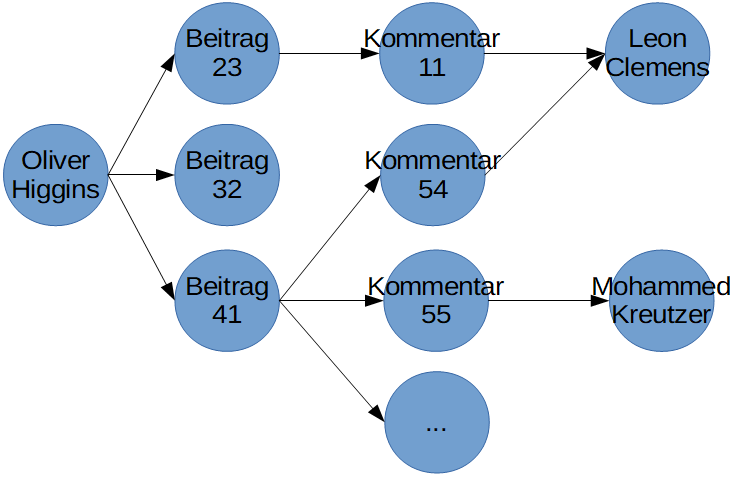
\includegraphics[width=0.6\textwidth]{images/graph.png}
	\caption{Graph zur Kommentiert-Von-Beziehung zwischen Oliver Higgins und Leon Clemens}
\end{figure}

Für die Statistik \grqq Mitglied wurde von anderes Mitglied so oft kommentiert\grqq{} ist es wichtig die Anzahl der Wege zwischen Oliver Higgins und Leon Clemens zu zählen. Diese Funktionalität unterstützt OQGRAPH nicht \cite{OQGRAPH-Examples}. Es ist nur möglich zu ermitteln, welcher Pfad der kürzeste ist oder welche Knoten von welchem Knoten aus erreichbar sind.

\begin{figure}[h]
	\centering
	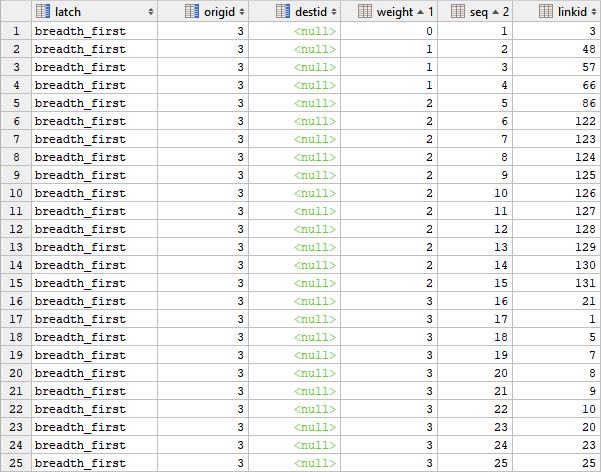
\includegraphics[width=0.7\textwidth]{images/oqgraph-select.png}
	\caption{SQL-Select, wobei origid = 3 hier Oliver Higgins: \newline
		\texttt{SELECT * FROM oq\_graph WHERE latch = 'breadth\_first'\newline AND origid = 3 AND weight < 4}
	}
\end{figure}

Das Ergebnis der Breitensuche stellt uns die im Rahmen der Breitensuche erreichten Knoten dar. Anhand des Vorwissens, dass die origid ein Mitglied ist und in unserem Anwendungsbeispiel es nur Beziehungen der Art Mitglied-Zu-Beitrag, Beitrag-Zu-Kommentar und Kommentar-Zu-Beitrag gibt, können wir darauf schließen, dass die erreichten Knoten mit dem Gewicht (weight) Mitgliedsknoten sein müssen. Wenn jetzt noch eine weitere Beziehung, beispielsweise \grqq Kommentar-Zu-Kommentar\grqq{} hinzukommt, ist ein solcher Schluss nicht mehr möglich. In diesem Fall müsste nach den gefundenen Knoten-IDs nach Treffern in den jeweiligen Knoten-Tabellen gesucht werden.

Das Ergebnis der Anfrage gibt außerdem auch andere Knoten anderer Gewichtungen an. Auch hier lässt sich aus der Gewichtung theoretisch schließen, dass es sich bei den Knoten der Gewichtung 1 um Beitragsknoten und bei Knoten der Gewichtung 2 um Kommentarknoten handelt. Es geht jedoch nicht hervor, in welcher Beziehung die Knoten zueinander stehen. So lässt sich ein Kommentar nicht eindeutig einem Mitglied zuordnen. Hier wäre also eine Tiefensuche sinnvoll, die OQGRAPH zur Zeit jedoch nicht unterstützt.

Auf Grund von fehlenden, für eine Graph-Datenbank jedoch essentielle, Funktionalitäten musste also auf reguläre SQL-Befehle zurückgegriffen werden. Besonderheiten in der Speicherung ergaben sich durch die Formulierung aller Elemente als Knoten, sowie die Speicherung der Beziehungen zwischen den Elementen als Kanten in einer gesonderten, relationalen Tabellen. Auf diese Weise werden jedoch Normalformen verletzt, wodurch es zu Anomalien kommen kann.

\subsection{Fazit}

OQGRAPH kam bei der Realisierung des Gästebuch-Clients nicht zum Einsatz. Grund hierfür ist, dass OQGRAPH eine Erweiterung eines relationalen Datenbanksystems ist. Für viele Abfragen eigneten sich einfache SQL-Abfragen ohne Bezug zu OQGRAPH besser. Da es in OQGRAPH von Grund auf nicht möglich ist Knoten anhand ihres Typs in unterschiedlichen Rekursionsstufen zu filtern und anschließend zu traversieren, wäre eine Umsetzung der Abfragen in OQGRAPH äußerst komplex und definitiv nicht praktikabel gewesen. Die Erweiterung OQGRAPH eignet sich deshalb nur für die Anwendungsfälle, in denen eine Betrachtung von speziellen Knoten- und Kanten-Typen nicht erforderlich ist.

\newpage
\setcounter{chapter}{4}
\setcounter{section}{0}
\section{MariaDB mit OQGRAPH}%Graph-Datenbanken im praktischen Einsatz: OLAP (chapter)
In diesem Abschnitt wird auf die Performanz von OLAP-Anwendungen in MariaDB-Datenbanksysteme mit OQGRAPH als Erweiterung eingegangen. Als OLAP-Testszenario werden Profile aus Datensätzen verschiedener Plattformen herangezogen. Diese Profile dienen fortlaufend als Knoten. Diese Knoten werden dann in weiteren Datensätzen über Kanten miteinander verbunden. Diese Kanten beinhalten außerdem zusätzliche Informationen, wie die Art der Beziehung, sowie ein Datum.

Die Daten sind den Plattformen \emph{Facebook}, \emph{Wikipedia}, \emph{Epinions}, \emph{YouTube} und \emph{LifeJournal} zugeordnet. Die entsprechenden Datensätze beinhalten alle eine unterschiedliche Anzahl an Knoten und Kanten.

\subsection{Implementierung der Datenbanken}

Für die Performanztests von MariaDB mit der OQGRAPH-Erweiterung wird der zur Verfügung stehende Cluster genutzt. Details zur Installation von MariaDB und der OQGRAPH-Erweiterung können dem Abschnitt \ref{Installation} entnommen werden. Es wird also ein bereits bestehendes MariaDB-Datenbanksystem genutzt, welches bis hierhin nur für die Implementierung der OLTP-Anwendung genutzt wurde. Um die Performanztests nicht zu verfälschen, wurde das MariaDB-Datenbanksystem für die Dauer der Tests nicht anderweitig genutzt.

Um die Datensätze voneinander zu abstrahieren und um die Performanztests voneinander unabhängig durchzuführen, wurde für jede Plattform jeweils eine Datenbank angelegt. In den fünf Datenbanken befinden sich jeweils zwei Tabellen.

Die Tabelle \emph{profil} beinhaltet alle Profile aus den Datensätzen der jeweiligen Plattformen. Jede Zeile in der Tabelle stellt hierbei einen Knoten dar. Dabei stellt die Tabelle \emph{profil} noch weitere Informationen zum Knoten zur Verfügung, wie den Vor- und Nachnamen, das Geschlecht, das Geburtsdatum und das Land. Das Land wurde noch indexiert, welches bei den Performance Messungen zur Anwendung kommt.

In der Tabelle \emph{oq\_backing} werden die Kantenbeziehungen zwischen den einzelnen Knoten gespeichert. Dabei folgt die Tabelle der Namenskonvention der OQGRAPH-Erweiterung. Die Spalte \emph{origid} referenziert hierbei auf den Ausgangsknoten, von dem eine gerichtete Kante zum Zielknoten ausgeht, welcher in \emph{destid} referenziert wird. Außerdem werden in den Spalten \emph{rtype} und \emph{date} weitere Informationen zur Kantenbeziehung gespeichert.

Für den Import der Zeilen aus den CSV-Datensätzen in die Datenbank wurde die Datenbank-IDE DataGrip genutzt. Beim CSV-Import wandelt die DataGrip-IDE die CSV-Datei in mehrere Insert-SQL-Statements um und führt diese Statements in der ausgewählten Datenbank aus. So wurden schließlich alle Zeilen aus den CSV-Dateien in die Datenbank importiert.

Die Anzahl der Zeilen in den Tabellen der verschiedenen Datenbanken kann der folgenden Auflistung entnommen werden.

\begin{center}
	\begin{tabular}{l|l l l l l }
		& Facebook & Wikipedia & Epinions & YouTube & LifeJournal \\
		\hline
		profil & 4.039 & 7.115 & 75.879 & 1.134.890 & 3.997.962 \\
		oq\_backing & 88.234 & 100.762 & 405.740 & 2.987.624 & 34.681.189 \\
	\end{tabular}
\end{center}

\subsection{Versuchsaufbau und Metriken}

Im Rahmen des Performanztests wird die Dauer einer einzelnen Operation als Metrik herangezogen. Hierbei wird die Zeit gemessen, die eine Operation in Form eines SQL-Statements benötigt. Hierbei kann es aber auch zu ausreißenden Beobachtungen kommen. Ausreißer können entstehen, weil das MariaDB-Datenbanksystem eine SQL-Abfrage nicht immer gleich und deshalb diese nicht immer über eine konstant gleichbleibende Dauer ausführt.

Es ist daher wichtig den Einfluss von Ausreißern möglichst zu minimieren. Aus diesem Grund werden die Messungen mehrmals durchgeführt und anschließend der durchschnittliche Zeitbedarf berechnet. Je nach Zugriffsart finden weitere Messungen statt. So werden bei Projektionen und Selektionen unterschiedliche Stellen der Tabellen abgefragt, da Abfragen auf den Beginn oder das Ende der Tabelle die Messungen verfälschen würde.

Die Mess-Vorgänge wurden in SQL-Prozeduren definiert. Diese Prozeduren übernehmen die Zeitmessung, die Speicherung der Messwerte, sowie die Ermittlung des Durchschnittes. Die Messergebnisse werden dabei in einer weiteren Tabelle \emph{analysis} gespeichert, die auf jeder Datenbank erstellt wurde. Die Prozeduren werden dann mittels des \emph{CALL}-SQL-Befehls aufgerufen.

\subsection{Annahmen}

\subsection{Performance-Messung}

\subsubsection{Projektion und Selektion}
Da OQGRAPH lediglich die Traversierung von Knoten ermöglicht sind die in diesem Kapitel durchgeführten Leistungstests keine Evaluierung des Graphsystems sondern der darunterliegenden relationalen Datenbank. Ein Ansatz, den Zugriff nur über die Kantentabelle zu ermöglichen, um so einen Anbindung an OQGRAPH zu simulieren wurde verworfen. Da die Performance unnötig leiden würde, da die Datenknotentabelle in jedem Fall gejoined werden muss. Gleichzeitig gibt es auch keine Vorteile, da der Primary Key der Datentabelle mit dem Knotenwert in der Backingtabelle identisch ist. Des Weiteren könnten die Ergebnisse verfälscht werden, wenn ein Datensatz kein Bestandteil einer Beziehung ist, sprich es existiert keine Kante zu diesem Datensatz.

Bei der Selektion anhand von Primärschlüsseln wurde eine Messung mit dem erstem (ID = 1) Datensatz durchgeführt. Es folgend weitere Messungen in tausender Schritten (ID + 1000) bis das Ende der Tabelle erreicht wird. So lässt sich sicherstellen das dass das Mittelmaß der Messungen auch realistisch ist.

Folgende \lstinline{SELECT} Statements wurden ausgeführt:
\begin{lstlisting}
-- Nur der Primaerschlussel
SELECT id FROM profil WHERE id = x;
-- Das Vollstaendige Profil
SELECT * FROM profil WHERE id = x;
\end{lstlisting}

Abbildung \ref{fig:NutzerPk} zeigt die Ergebnisse auf den unterschiedlichen Datenbanken. Es lassen sich nur leichte Schwankungen bei den Messwerten feststellen. Die Größe der Datenbank ist daher eher unerheblich, tendenziell benötigen Selektion mit sämtlichem Attributen mehr Zeit, ist aber durchaus vernachlässigbar.
\begin{figure}[h]
	\centering
	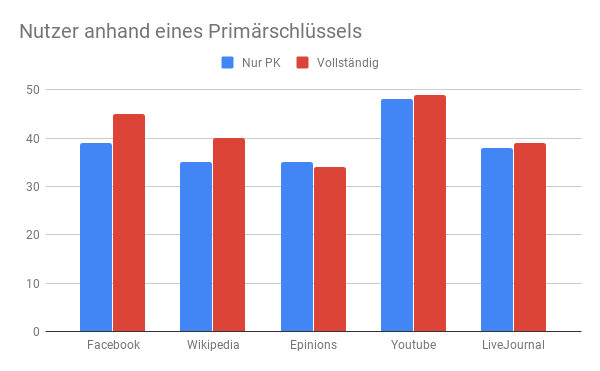
\includegraphics[width=\textwidth]{images/NutzerPk.png}
	\caption{Messergebnisse zur Selektion eines Nutzers anhand des Primärschlüssels}
	\label{fig:NutzerPk}
\end{figure}

Bei der Selektion anhand eines Nichtprimärschlüssels offenbarten sich zwei Probleme. Da auf den selektierten Attributen kein \emph{Unique Constraint} definiert ist, benötigen große Datenbanken exponentiell länger für die selbe Anfrage, da ein kompletter Scan durchgeführt werden muss. Dementsprechend ist die Vergleichbarkeit nicht mehr gewährleistet. Dieses Problem ließ sich durch eine \lstinline{LIMIT 1} Klausel lösen.

Problematisch war auch, dass sich im Gegensatz zum Primärschlüssel die Anzahl der Abfragen nur schwer begrenzen lässt, da sich nicht mit fest vorgegeben Parameter arbeiten lässt. Stattdessen liefert ein zuvor definierter Cursor, welcher \lstinline{DISTINCT} Werte des entsprechenden Attributs selektiert, die Parameter. Im Falle des indexierten Zugriff erübrigte sich das Problem von selbst, da die Anzahl der Länder in einem idealem Rahmen lagen. Bei dem nicht indexierten Zugriff wurde aber nach den Nachnamen gesucht, hier mussten die Parameter noch weiter eingeschränkt werden. Durch die Verwendung einer \lstinline{WHERE RAND()<=0.001} Klausel konnte der Parameterraum auf ein tausendstel reduziert werden.

Bei der Selektion mittels Nichtschlüsselattributen wurden folgenden \lstinline{SELECT} Statements ausgeführt:
\begin{lstlisting}
-- Anhand eines indexierten Attributes
SELECT * FROM profil WHERE country = v LIMIT 1;
-- Anhand eines nicht-indexierten Attributes
SELECT * FROM profil WHERE last = v LIMIT 1;
\end{lstlisting}

Abbildung \ref{fig:NutzerNPk} und Abbildung \ref{fig:NutzerNPkI} zeigt die Ergebnisse der nicht-indexierten und indexierten Selektion auf den unterschiedlichen Datenbanken. Es ist zu erkennen das bei einer Selektion die Performanz von sehr großen Datenbank stark leidet. Auch bei einem indexierten Zugriff nimmt die Performanz mit steigender Datenmenge ab, die benötigte Zeit ist aber dennoch wesentlich geringer.
\begin{figure}[h]
	\centering
	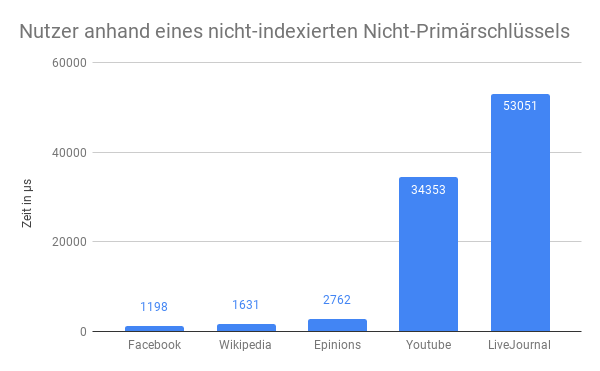
\includegraphics[width=\textwidth]{images/NutzerNPk.png}
	\caption{Messergebnisse zur Selektion eines Nutzers anhand eines Nicht-Primärschlüssels}
	\label{fig:NutzerNPk}
\end{figure}

\begin{figure}[h]
	\centering
	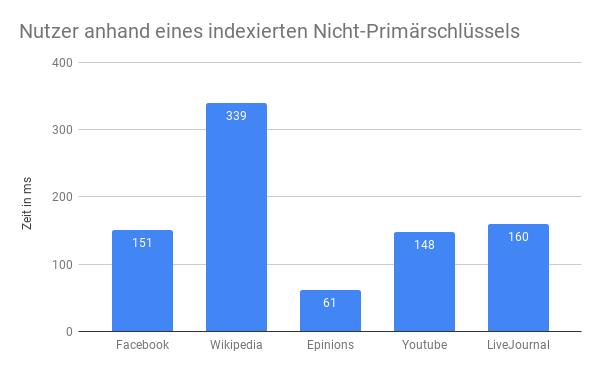
\includegraphics[width=\textwidth]{images/NutzerNPkI.png}
	\caption{Messergebnisse zur Selektion eines Nutzers anhand eines Nicht-Primärschlüssels}
	\label{fig:NutzerNPkI}
\end{figure}


\subsubsection{Aggregation}
Aus dem selben Grund wie bei Selektion und Projektion wurden auch bei diesen Tests ledigliche die relationalen SQL Datentabellen betrachtet.

Folgende Tests wurden durchgeführt:
\begin{enumerate}
	\item Anzahl aller Nutzer - Abbildung \ref{fig:AnzahlNutzer}
	\item Anzahl aller Beziehungen zwischen Nutzern - Abbildung \ref{fig:AnzahlBeziehung}
	\item Durchschnittliche Alters aller Nutzer - Abbildung \ref{fig:DurschAlter}
	\item Durchschnittliche Dauer aller Beziehung - Abbildung \ref{fig:DurschBeziehung}
\end{enumerate}

Folgende SQL Statements wurden durchgeführt:
\begin{lstlisting}
-- Anzahl Nutzer
SELECT COUNT(id) FROM profil;
-- Anzahl Beziehungen
SELECT COUNT(*) FROM oq_backing;
-- Durchschnittsalter
SELECT AVG(YEAR(NOW()) - YEAR(birth)) FROM profil;
-- Durchscnittsdauer Beziehungen
SELECT AVG(DATEDIFF(CURRENT_DATE, date)) FROM oq_backing;
\end{lstlisting}

Die Ergebnisse sind wenig überraschend, so steigt mit wachsender Datenmenge auch die benötigte Zeit. Je komplexer die Berechnung desto steiler der Anstieg. Da diese Operationen auf einer relationalen Tabelle ausgeführt wurden, machen sich auch die Vorteile eines solchen Models bemerkbar. Es ist davon auszugehen das spaltenweise SQL Aggregation wesentlich performanter ist, da nicht erst die Knoten geladen und deren Attribute extrahiert werden müssen.

\begin{figure}
	\centering
	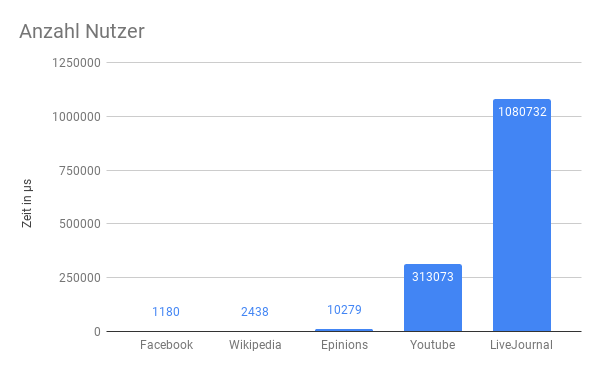
\includegraphics[width=\textwidth]{images/AnzahlNutzer.png}
	\caption{Messergebnisse zur Zählung sämtlicher Nutzeraccounts}
	\label{fig:AnzahlNutzer}
\end{figure}

\begin{figure}
	\centering
	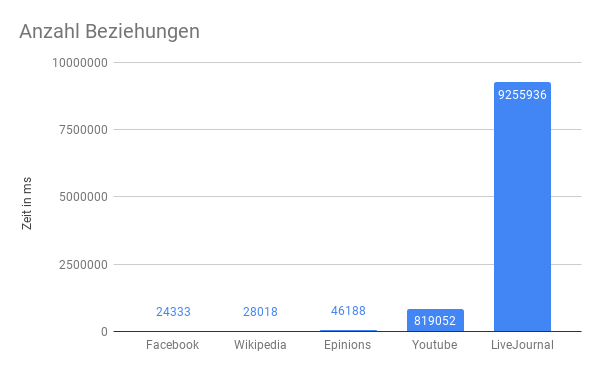
\includegraphics[width=\textwidth]{images/AnzahlBeziehung.png}
	\caption{Messergebnisse zur Zählung bestehender Beziehungen}
	\label{fig:AnzahlBeziehung}
\end{figure}

\begin{figure}
	\centering
	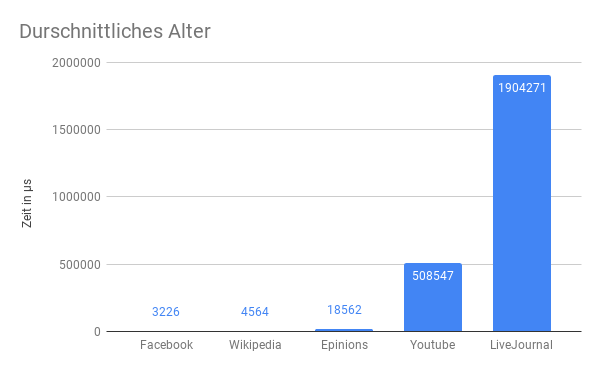
\includegraphics[width=\textwidth]{images/DurschAlter.png}
	\caption{Messergebnisse zur Berechnung des Durchschnittsalter}
	\label{fig:DurschAlter}
\end{figure}

\begin{figure}
	\centering
	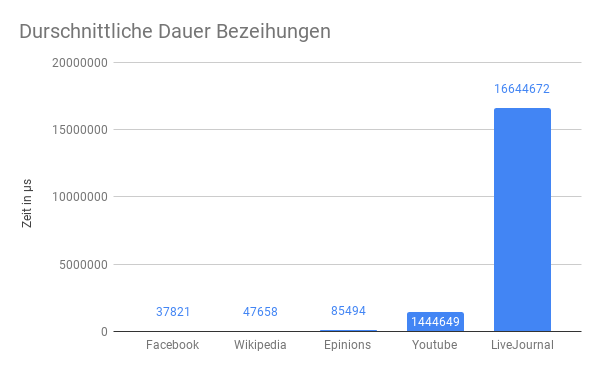
\includegraphics[width=\textwidth]{images/DurschBeziehung.png}
	\caption{Messergebnisse zur Berechnung der Dauer eine durchschnittlichen Beziehung}
	\label{fig:DurschBeziehung}
\end{figure}

\newpage

\subsubsection{Traversierung}
Für die Traversierung wird OQGRAPH-Engine verwendet, aber zuerst für Benutzung der OQGRAPH werden spezialle Vorbereitungstabellen erstellt, bei dessen Aufbau nur die relationalen Befehlen durchgeführt wurden.

Folgende Tests wurden durchgeführt:
\begin{enumerate}
	\item Erstellung der OQGRAPH Tabellen \ref{fig:facevor}
	\ref{fig:wikivor}
	\ref{fig:epinvor}
	\ref{fig:youtubvor}
	\ref{fig:LiJouvor}
	\item Transitive Suche in Facebook
	\ref{fig:face}
	\item Transitive Suche in Wikipedia
	\ref{fig:wiki}
	\item Transitive Suche in Epinions 
	\ref{fig:epin}
	\item Transitive Suche in Youtube 
	\ref{fig:youtub}
	\item Transitive Suche in LiveJournal 
	\ref{fig:LiJou}
\end{enumerate}


Folgende SQL Statements (nur die wichtige SQL Befehlen) wurden durchgeführt:
\begin{lstlisting}
-- Vorbereitung Tabelle der Business Kontakten
SELECT * FROM oq_backing WHERE rtype = "BUSINE";

-- Vorbereitung Tabelle der auslaendischen Kontakten
SET @land = 'BE';
SELECT DISTINCT * FROM 
(SELECT b1.origid, b1.destid FROM oq_backing b1 INNER JOIN
 profil p1 ON b1.destid = p1.id WHERE p1.country <> @land
UNION
SELECT b2.origid, b2.destid FROM oq_backing b2 INNER JOIN
 profil p2 ON b2.origid = p2.id WHERE p2.country <> @land
UNION
SELECT b3.origid, b3.destid FROM oq_backing b3 INNER JOIN
 profil p3 ON b3.origid = p3.id WHERE p3.id = sID
UNION
SELECT b4.origid, b4.destid FROM oq_backing b4 INNER JOIN
 profil p4 ON b4.destid = p4.id WHERE p4.id = sID);
 
-- Suche nach Kontakten
SELECT * FROM oq_graph WHERE latch='breadth_first' AND
 origid="start ID Knote" AND weight <= "Tiefe gerichtet" AND
  weight>0;
  
-- Suche nach Business Kontakten
SELECT * FROM oq_graph_business WHERE latch='breadth_first'
 AND origid="start ID Knote" AND weight <= "Tiefe gerichtet"
  AND weight>0;
  
-- Suche nach auslaendischen Kontakten
SELECT * FROM oq_graph_ausland WHERE latch='breadth_first'
 AND origid="start ID Knote" AND weight <= "Tiefe gerichtet"
  AND weight>0;
\end{lstlisting}


\begin{figure}
	\centering
	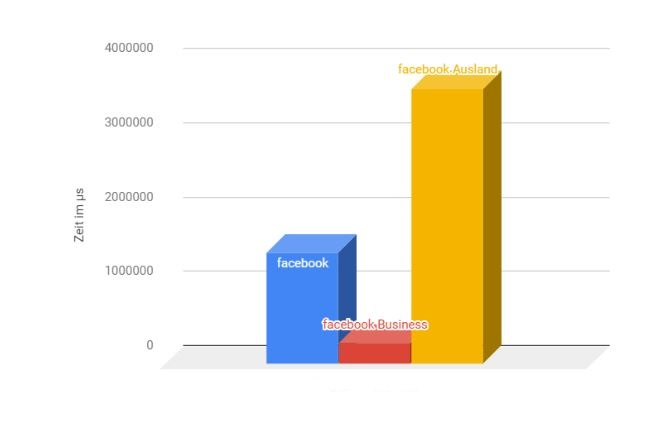
\includegraphics[width=\textwidth]{images/facevor.jpg}
	\caption{Messergebnisse zur Vorbereitung OQGRAPH Tabelle Facebook}
	\label{fig:facevor}
\end{figure}

\begin{figure}
	\centering
	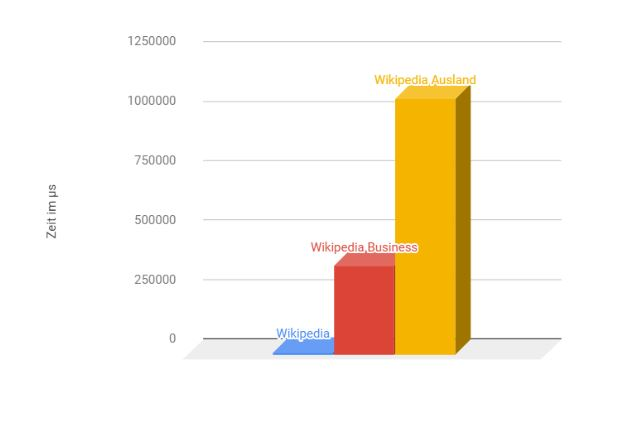
\includegraphics[width=\textwidth]{images/wikivor.jpg}
	\caption{Messergebnisse zur Vorbereitung OQGRAPH Tabelle Wikipedia}
	\label{fig:wikivor}
\end{figure}

\begin{figure}
	\centering
	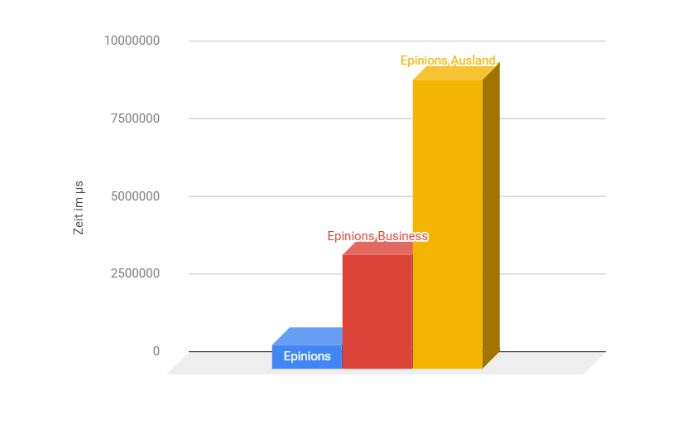
\includegraphics[width=\textwidth]{images/epinvor.jpg}
	\caption{Messergebnisse zur Vorbereitung OQGRAPH Tabelle Epinions}
	\label{fig:epinvor}
\end{figure}

\begin{figure}
	\centering
	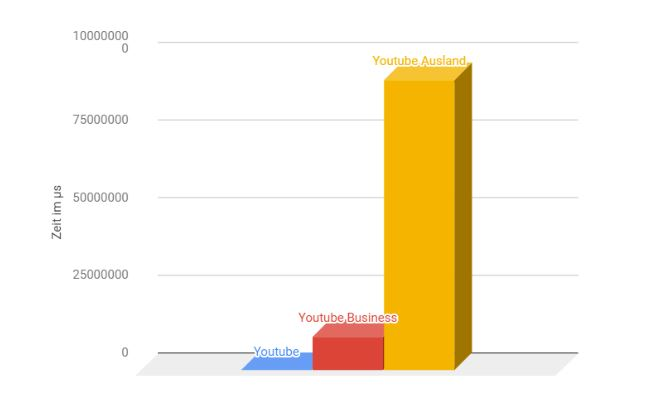
\includegraphics[width=\textwidth]{images/youtubvor.jpg}
	\caption{Messergebnisse zur Vorbereitung OQGRAPH Tabelle YouTube}
	\label{fig:youtubvor}
\end{figure}

\begin{figure}
	\centering
	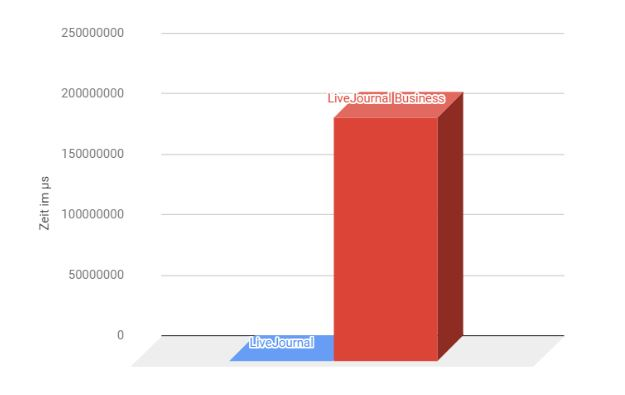
\includegraphics[width=\textwidth]{images/LiJouvor.jpg}
	\caption{Messergebnisse zur Vorbereitung OQGRAPH Tabelle LiveJournal}
	\label{fig:LiJouvor}
\end{figure}

Die Ergebnisse sind ganz erwarten, dass je größer die Datebanken sind, desto mehr die Zeit wird für die Erstellung der Tabellen benötigt und im Fall der QOGRAPH ausländischen Tabellen im LiveJournall ist Aufwand wegen mehreren JOIN Befehelen wirklich zu groß um die Ergebnisse zu berechnen.
Auch geht es um die kleine Daten im Tabelle "Facebook", darum kann die Tabelle manchmal  für die geschäftlichen Kontakten ein bisschen schneller erstellt werden.  


\begin{figure}
	\centering
	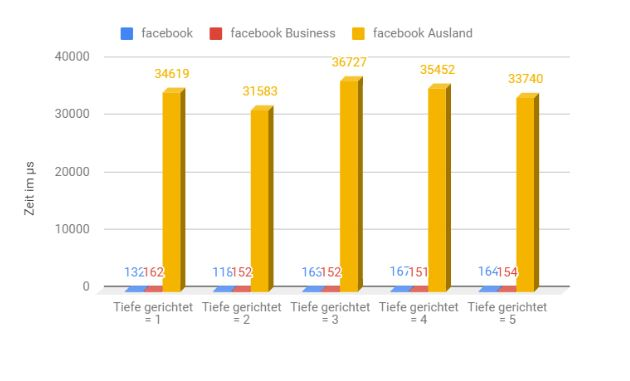
\includegraphics[width=\textwidth]{images/face.jpg}
	\caption{Messergebnisse nach Tiefenstufen in Tabelle Facebook}
	\label{fig:face}
\end{figure}

\begin{figure}
\centering
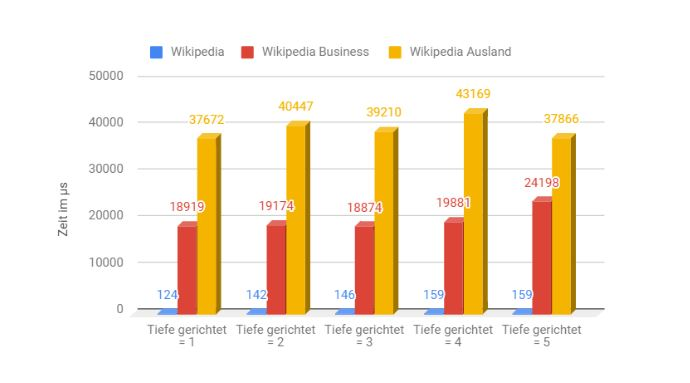
\includegraphics[width=\textwidth]{images/wiki.jpg}
\caption{Messergebnisse nach Tiefenstufen in Tabelle Wikipedia}
\label{fig:wiki}
\end{figure}

\begin{figure}
	\centering
	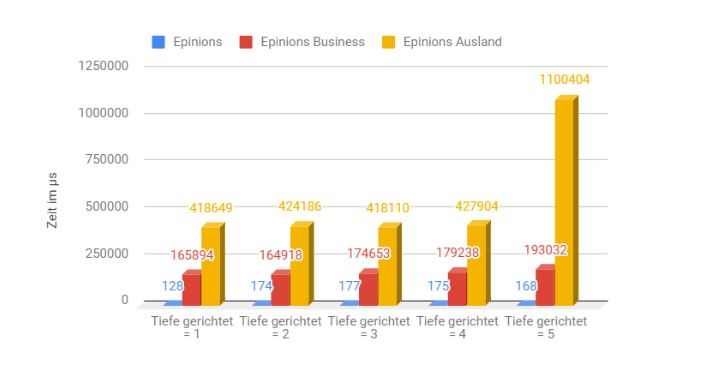
\includegraphics[width=\textwidth]{images/epin.jpg}
	\caption{Messergebnisse nach Tiefenstufen in Tabelle Epinions}
	\label{fig:epin}
\end{figure}

\begin{figure}
	\centering
	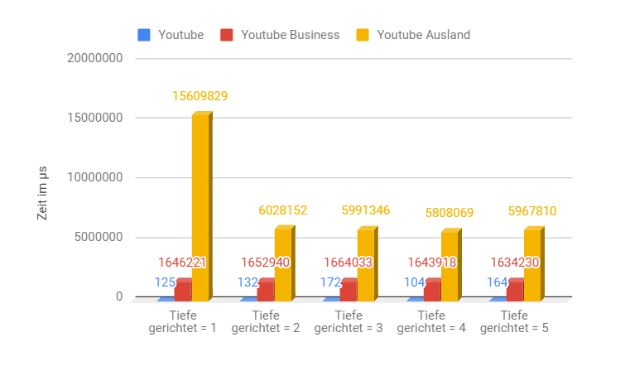
\includegraphics[width=\textwidth]{images/youtub.jpg}
	\caption{Messergebnisse nach Tiefenstufen in Tabelle YouTube}
	\label{fig:youtub}
\end{figure}

\begin{figure}
	\centering
	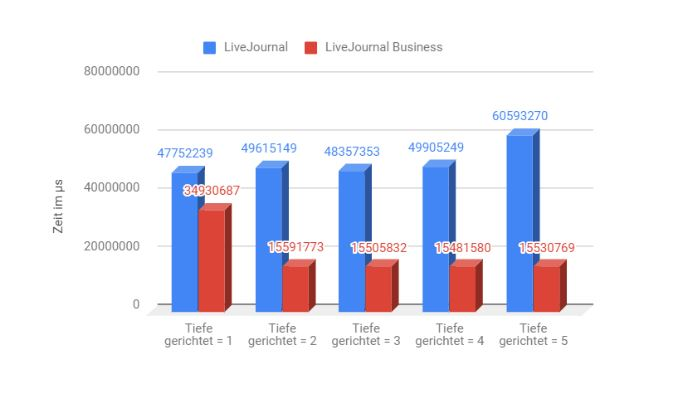
\includegraphics[width=\textwidth]{images/LiJou.jpg}
	\caption{Messergebnisse nach Tiefenstufen in Tabelle LiveJournal}
	\label{fig:LiJou}
\end{figure}

Allgemeine kann man feststellen, dass die Bearbeitungszeit für jede Transitive Suche vom Tiefstufen unabhängig ist. Manchmal ist bei einigen Suchen die Bearbeitungszeit groß,  z.B als auf dem Diagramm der Epinions im Tiefestufe 5, aber manchmal ist es auch in der Tiefestufe 1 auch, als in Youtube, darum hängt die Bearbeitungszeit von etwas Anderes als Tiefstufen ab. Und trotz vielen Zahlen der Knoten im Livejournal bleibt diese Tendenz fast gleich.

\subsection{Fazit}
Ebenso wie bei der OLTP Anwendung erfordert der begrenzte Funktionsumfang von OQGRAPH ein Ausweichen auf relationales SQL. Lediglich bei der Traversierung von Knoten kamen Funktionalitäten von OQGRAPH zum Einsatz, allerdings musste auch hier mit Workarounds gearbeitet werden um die Limitierung der homogenen Kanten zu umgehen. Die Performance selbst kann dabei mit konkurrierenden Graphdatenbanken mithalten. Positiv bemerkbar hat sich das koexistierende relationale Datenmodel hingegen bei der Aggregation gemacht, hier kamen die Vorteile von SQL zum Einsatz.

\newpage
\setcounter{chapter}{5}
\setcounter{section}{0}
\subsection{Zusammenfassung}

OQGRAPH ist eine Erweiterung von MariaDB, die sich sehr leicht installieren lässt. Es erweitert die relationale Datenbank und SQL um spezielle Abfragen im Bezug auf Graphen. Es nutzt und erzeugt selbst relationale Datenstrukturen. Die Traversierung ist dabei auch in hohen Rekursionsstufen sehr schnell und zuverlässig. Jedoch ist eine Unterteilung von Knoten und Kanten in bestimmte Typen nur über reguläre SQL-Abfragen möglich, auf die OQGRAPH aufsetzt. So steigt die Komplexität um die Nutzung von OQGRAPH.

Die Erweiterung OQGRAPH eignet sich daher noch für Anwendungsfälle, in denen Knoten und Kanten nicht in ihren Typen unterschieden werden oder bereits gefiltert wurden. In solchen Anwendungsfällen kann OQGRAPH die Komplexität reduzieren, da mittels der Traversierung hier keine komplexen SQL-JOIN-Verflechtungen mehr notwendig sind. In den Anwendungsfällen, in denen Knoten und Kanten in ihren Typen unterschieden werden, ist eine entsprechende Vorverarbeitung notwendig. Eine Selektion von Knoten in einer Kette von speziellen Typen, wie im Beispiel des Gästebuches, ist nur unter sehr hohem Aufwand oder mittels fehleranfälliger Workarounds möglich.

\subsection{Pros}
\begin{itemize}
	\setlength\itemsep{-0.5em}
	\item Erweiterung der relationalen Datenbankwelt
	\item Sehr schnelle Traversierung
	\item Durch Traversierung Reduktion der Komplexität, keine verschachtelten SQL-JOIN-Abfragen mehr notwendig
	\item Sehr leichte Installation
	\item Viele graph-typische Verfahren implementiert
\end{itemize}

\subsection{Cons}
\begin{itemize}
	\setlength\itemsep{-0.5em}
	\item Bei Traversierung keine Unterscheidung von Knoten- und Kanten-Typen möglich
	\item Keine Wegangabe bei der Traversierung
	\item Kein Zählen von möglichen Wegen zwischen zwei Knoten möglich
	\item OQGRAPH spezifische Speicherung von Knoten und Kanten kann Normalformen verletzen - Anomalien sind möglich
\end{itemize}

\newpage

% loads the fancy pagestyle for register part
% set the pagestyle to fancy
\pagestyle{fancy}

\fancyhf{}% clear all fields
  % define the header
  \fancyhead[L]{\leftmark}% left header
  \fancyhead[R]{\HEADER}% right header
  \renewcommand{\headrulewidth}{0.4pt}% top line

  % define the footer
  \fancyfoot[L]{\AUTHOR}% left footer
  \fancyfoot[R]{\pagemark}% right footer
  \renewcommand{\footrulewidth}{0.6pt}% bottom line

  % redefine the chaptermark to have '1. Chaptername' and not 'CHAPTER 1.
  % CHAPTERNAME'
  \renewcommand{\chaptermark}[1]{\markboth{\thechapter.\ #1}{}}

% override the plain style
\fancypagestyle{plain}{%
\fancyhf{}% clear all fields
  % define the header
  \renewcommand{\headrulewidth}{0.0pt}% top line

  % define the footer
  \fancyfoot[L]{\AUTHOR}% left footer
  \fancyfoot[R]{\pagemark}% right footer
  \renewcommand{\footrulewidth}{0.6pt}% bottom line
}


% #####
% # load the appendix from the files
% #####
\appendix
\chapter{Anhang}
\section{Schema für die OQGRAPH Backing-Tabelle}\label{schemaBacking}
\begin{lstlisting}
CREATE TABLE oq2_backing (
  origid INT UNSIGNED NOT NULL, 
  destid INT UNSIGNED NOT NULL, 
  weight DOUBLE NOT NULL, 
  PRIMARY KEY (origid, destid), 
  KEY (destid)
);	
\end{lstlisting}
\section{Schema für die OQGRAPH API-Tabelle}\label{schemaApi}
\begin{lstlisting}
CREATE TABLE oq_graph
ENGINE=OQGRAPH 
data_table='oq_backing' 
origid='origid'
destid='destid' 
weight='weight';
\end{lstlisting}
Für MariaDB Versionen älter als 10.1.2 müssen die Attribute manuell spezifiziert werden.
\begin{lstlisting}
CREATE TABLE oq_graph (
  latch VARCHAR(32) NULL,
  origid BIGINT UNSIGNED NULL,
  destid BIGINT UNSIGNED NULL,
  weight DOUBLE NULL,
  seq BIGINT UNSIGNED NULL,
  linkid BIGINT UNSIGNED NULL,
  KEY (latch, origid, destid) USING HASH,
  KEY (latch, destid, origid) USING HASH
) ENGINE=OQGRAPH 
data_table='oq_backing' 
origid='origid' 
destid='destid' 
weight='weight';	
\end{lstlisting}
\section{Installationsscript der OLTP Anwendung}
\lstset{
	columns=fullflexible,
	breaklines=true,
	postbreak=\mbox{\textcolor{red}{$\hookrightarrow$}\space},
}
%\lstinputlisting[language=SQL]{appendix/oltp_create.log}
\section{Messergebnisse des OLAP Systems}
\begin{tabularx}{\textwidth}{X X X X X X}
	\textbf{Test Case}    & \textbf{Facebook}  & \textbf{Wikipedia} & \textbf{Epinions} & \textbf{Youtube} & \textbf{LiveJournal} \\
	\hline
	Selektion PK &	39&	35&	35&	48&	38\\
	PK (Vollständig)&	45&	40&	34&	49&	39\\
	NPK&	1198&	1631&	2762&	34353&	53051\\
	indexierter NPK&	151&	339&	61&	148&	160\\
	Anz. Nutzer&	1180&	2438&	10279&	313073&	1080732\\
	Anz. Beziehungen&	24333&	28018&	46188&	819052&	9255936\\
	AVG Alter&	3226&	4564&	18562&	508547&	1904271\\
	AVG Beziehung&	37821&	47658&	85494&	1444649&	16644672\\
\end{tabularx}

\begin{tabularx}{\textwidth}{X X X X X X X}
	\textbf{Test Case} & \textbf{OQ GRAPH Tab.}    & \textbf{Tiefe=1}  & \textbf{Tiefe=2} & \textbf{Tiefe=3} & \textbf{Tiefe=4} & \textbf{Tiefe=5} \\
	\hline
	Facebook&	1499107&	132& 118& 163&	167& 164\\
	Facebook Business&	281034&	162&	152&	152& 151&	154\\
	Facebook Ausland &	3707682&	34619&	31583&	36727&	35452&	33740\\
	Wikipedia&	7818&	124&	142&	146&	159&	159\\
	Wikipedia Business&	372839&	18919&	19174&	18874&	19881&	24198\\
	Wikipedia Ausland &	1074857&	37672&	40447&	39210&	43169&	37866\\
	Epinions&	769848&	128&	174&	177&	175&	168\\
	Epinions Business&3677083&	165894&	164918&	174653&	179238&	193032\\
	Epinions Ausland &	9328571 &418649&	424186&	418110&	427904&	1100404\\
	YouTube&8104&	125&	132&	172&	104&	164\\
	YouTube Busines&	10888958&	1646221&1652940&	1664033&	1643918&	1634230\\
	YouTube Ausland &93601019&15609829&	6028152	&5991346&	5808069&	5967810\\
	Live Journal&7988	&	47752239&	49615149&	48357353&	49905249&	60593270\\
	Live Journal Business&201885673	&	34930687&	15591773&	15505832&	15481580&	15530769\\
\end{tabularx}


% #####
% # list of table, list of figures, and list of listings in ToC
% #####
\newpage
\addcontentsline{toc}{chapter}{Abbildungsverzeichnis}
\listoffigures
\newpage
\addcontentsline{toc}{chapter}{Tabellenverzeichnis}
\listoftables
\newpage
\addcontentsline{toc}{chapter}{Listings}
\lstlistoflistings

% #####
% # List of Abbreviations
% #####
\phantomsection 
\addcontentsline{toc}{chapter}{Abkürzungsverzeichnis}
\renewcommand\refname{Abkürzungsverzeichnis} 
\chapter*{Abkürzungsverzeichnis}
\begin{acronym}[RDBMS] % längste Abkürzung steht in eckigen Klammern
    \setlength{\itemsep}{-\parsep} % geringerer Zeilenabstand
    \acro{API}{Application Programming Interface}
    \acro{BASE}{Basically Available, Soft State, Eventual Consistency}
    \acro{BG}{Barahmand Ghandeharizadeh}
    \acro{CAP}{Consistency Availibiltiy Partition Tolerance}
    \acro{CLI}{Command-Line Interface}
    \acro{CPU}{Central Processing Unit}
    \acro{CRUD}{Create, Read, Update, Delete}
    \acro{DBA}{Datenbankadministrator}
    \acro{DBS}{Datenbanksystem}
    \acrodefplural{DBS}[DBS]{Datenbanksysteme}
    \acrodefplural{HDD}[HDDs]{Hard Disk Drive}
    \acrodefplural{SSD}[SSDs]{Solid State Drive}
    \acro{DNS}{Domain Name System}
    \acro{DTD}{Document Type Definition}
    \acro{GUI}{Graphical User Interface}
    \acro{HDD}{Hard Disk Drive}
    \acro{IP}{Internet Protocol}
    \acro{JDBC}{Java Database Connectivity}
    \acro{JSON}{JavaScript Object Notation}
    \acro{NoSQL}{Not only SQL}
    \acro{OLTP}{Online Transaction Processing}
    \acro{RDBMS}{Relational Database Management System}
    \acro{RFC}{Request For Comments}
    \acro{SLA}{Service Level Agreement}
    \acro{SPEC}{Standard Performance Evaluation Corporation}
    \acro{SQL}{Structured Query Language}
    \acro{SSD}{Solid State Drive}
    \acro{TPC}{Transaction Processing Performance Council}
    \acro{UML}{Unified Markup Language}
    \acro{XML}{Extensible Markup Language}
    \acro{YCSB}{Yahoo! Cloud Serving Benchmark}
\end{acronym}

\newpage

% #####
% # load the bibliography
% #####
\bibliography{bibliography}

% #####
% # load the sworn declaration
% #####
%\chapter*{Eidesstattliche Erklärung}\markboth{Eidesstattliche Erklärung}{}
  \addcontentsline{toc}{chapter}{Eidesstattliche Erklärung}
Ich versichere an Eides Statt durch meine eigenhändige Unterschrift, dass
ich die vorliegende Arbeit selbstständig und ohne fremde Hilfe angefertigt
habe. Alle Stellen, die wörtlich oder dem Sinn nach auf Publikationen oder
Vorträgen anderer Autoren beruhen, sind als solche kenntlich gemacht.
Ich versichere außerdem, dass ich keine andere als die angegebene
Literatur verwendet habe. Diese Versicherung bezieht sich auch auf alle in
der Arbeit enthaltenen Zeichnungen, Skizzen, bildlichen Darstellungen und
dergleichen.
\\
\\
Die Arbeit wurde bisher keiner anderen Prüfungsbehörde vorgelegt und
auch noch nicht veröffentlicht.
\vspace{3cm}

\centering
\begin{tabular}{p{10mm}>{\centering\arraybackslash}p{50mm}p{10mm}
>{\centering\arraybackslash}p{50mm}p{10mm}}
&\textit{\large \TOWN,}&&& \\
&\textit{\large den \today}&&\hrulefill& \\
&\small Ort, Datum&&\small \AUTHOR&
\end{tabular}
% end of the document
\end{document}
